\documentclass[a4paper,fleqn]{cas-sc}

\usepackage[numbers,sort&compress]{natbib}
\usepackage{amsmath,amssymb,amsfonts}
\usepackage{graphicx}
\usepackage{booktabs}
\usepackage{array}
\usepackage{url}
\renewcommand{\sfdefault}{lmss}
\renewcommand{\ttdefault}{lmtt}
\usepackage{microtype}
\makeatletter
\newcommand{\tableinput}[1]{\@@input #1 }
\makeatother

\begin{document}
\let\WriteBookmarks\relax
\def\floatpagepagefraction{1}
\def\textpagefraction{.001}

% Short title and authors
\shorttitle{Exact SAT Solving and Baseline Comparisons for CBMP}
\shortauthors{T. D. Duc, H. M. Duc, and L. T. Hieu}

% Main title
\title[mode = title]{Exact SAT Solving and Comprehensive Baseline Comparisons for the Cyclic Bandwidth Minimization Problem}

% Authors
\author[1]{Truong Dinh Duc}
\ead{24021419@vnu.edu.vn}

\author[1]{Hoang Minh Duc}
\ead{24021411@vnu.edu.vn}

\author[1]{Le Trung Hieu}
\cormark[1]
\ead{24021475@vnu.edu.vn}

\address[1]{Faculty of Information Technology, VNU University of Engineering and Technology, 144 Xuan Thuy, Cau Giay Ward, Hanoi, 100000, Vietnam}

\cortext[1]{Corresponding author}

\begin{abstract}
The Cyclic Bandwidth Minimization Problem (CBMP) seeks a bijective labeling of the vertices of a graph with the positions of a cycle that minimizes the largest cyclic distance between the labels of adjacent vertices. Heuristic methods provide strong upper bounds for CBMP but do not certify optimality. We study exact SAT-based solving for CBMP and compare it with constraint programming (CP) and mixed integer linear programming (MIP) solvers. We formulate two SAT encodings of the decision problem $CB(G,\phi)\le B$: a pairwise encoding based on one-hot label variables and forbidden label pairs, and an order encoding based on threshold literals $[\phi(v)\ge k]$, cardinality constraints, and selector-guarded distance regions. Both encodings are solved by repeated SAT calls with binary search, and the pairwise encoding is additionally solved by an incremental descending search that keeps one solver instance alive. Rotation and reflection symmetries of the host cycle are removed by unit clauses. The baselines are IBM ILOG CPLEX CP Optimizer, Google OR-Tools CP-SAT, Gurobi, CPLEX MIP, and HiGHS. On 59 Harwell--Boeing instances with 24 to 245 vertices and a 300~s limit per instance, the order encoding certifies optimality for 23 instances (median 5.16~s), compared with 20 for CP-SAT, 16 for the pairwise encoding, 15 for incremental pairwise SAT, 12 for CPLEX CP, 7 for Gurobi and CPLEX MIP, and 1 for HiGHS; a two-solver portfolio of the order encoding and CP-SAT matches the 25-instance virtual best solver. CPLEX CP, however, dominates primal quality, returning the best upper bound on 57 of the 59 instances with a mean relative gap of only 0.5\% over the best-found bound. Incremental search cuts pairwise CNF construction time by 62.5\% and improves upper bounds on 29 instances, while symmetry breaking increases certified counts by up to 60\% and yields 1.84$\times$ to 4.38$\times$ geometric mean speedups across SAT and CP solvers.
\end{abstract}

\begin{keywords}
Cyclic bandwidth minimization \sep SAT encoding \sep Order encoding \sep Incremental SAT \sep Constraint programming \sep Mixed integer linear programming \sep Symmetry breaking
\end{keywords}

\maketitle

\section{Introduction}
\label{sec:intro}

Graph layout problems arrange the vertices of a graph on a target structure under different optimization objectives, with applications in VLSI design, interconnection networks, and sparse matrix computations~\citep{leung1984,hromkovic1992,duff1989}. In the classical bandwidth minimization problem (BMP), vertices receive distinct positions on a path and the objective is the largest distance between the positions of adjacent vertices. The \emph{Cyclic Bandwidth Minimization Problem} (CBMP) replaces the path by a cycle $C_n$, so distances wrap around the cycle~\citep{leung1984,lin1994}. The cyclic distance is not convex in the labels, which makes linear and constraint models of CBMP harder to write and to solve than those of BMP.

CBMP was introduced to model the design of ring interconnection networks~\citep{leung1984}. It has since been used as a model for VLSI design, data structure representations, code design, and the embedding of parallel computations into rings of processors~\citep{hromkovic1992,ren2020nils}. The decision version of CBMP is NP-complete~\citep{lin1994}. Early studies were mainly theoretical and established exact cyclic bandwidths for special graph classes and bounds for general graphs~\citep{hromkovic1992,lin1994}. Practical methods are mostly heuristics, including the tabu search $TS_{CB}$ of \citet{rodrigueztello2015}, the iterated three-phase search ITPS of \citet{ren2019}, and the new iterated local search NILS of \citet{ren2020nils}. These methods return upper bounds without a certificate of optimality. The only exact algorithm reported in this line of work is a branch-and-bound method that solves graphs with up to 40 vertices~\citep{romero2012}.

Boolean satisfiability (SAT) solving has become an effective exact approach for graph problems such as graph coloring, bandwidth coloring, and antibandwidth~\citep{handbooksat2021,prestwich2009,tamura2009}. A SAT approach reduces the optimization problem to a sequence of decision problems ``is there a labeling with cyclic bandwidth at most $B$?'', and a conflict-driven clause learning (CDCL) solver such as CaDiCaL~\citep{biere2024} answers each of them with a satisfying labeling or a proof of unsatisfiability. The smallest satisfiable $B$ is then a certified optimum.

This paper studies this approach for CBMP. Its contributions are the following.
\begin{enumerate}
    \item Two SAT encodings of the CBMP decision problem: a \emph{pairwise encoding} with one-hot label variables and forbidden label pairs, and an \emph{order encoding} with threshold literals, cardinality-based injectivity, and selector-guarded cyclic distance regions.
    \item Two solving schemes: repeated SAT calls with binary search for both encodings, and an incremental descending search for the pairwise encoding that adds only the clauses of the new bound to a persistent solver.
    \item Rotation and reflection symmetry-breaking constraints for the host cycle, applied uniformly to the SAT, CP, and MIP models.
    \item CP baselines in CPLEX CP Optimizer and OR-Tools CP-SAT, and a MIP baseline solved by Gurobi, CPLEX MIP, and HiGHS.
    \item An evaluation on 59 Harwell--Boeing instances under a 300~s limit, with figures produced by the \texttt{cnsplots} library~\citep{cnsplots}.
\end{enumerate}

The remainder of the paper is organized as follows. Section~\ref{sec:formulations} defines CBMP, reviews related work, and presents the MIP and CP baselines. Section~\ref{sec:sat} presents the SAT encodings, the solving schemes, and symmetry breaking. Section~\ref{sec:experiments} reports the computational experiments. Section~\ref{sec:conclusion} concludes the paper.

\section{Background and Exact Baselines}
\label{sec:formulations}

\subsection{Problem Definition}

Let $G=(V,E)$ be a simple undirected graph with vertex set $V=\{1,\dots,n\}$ and edge set $E$, where $|E|=m$. A labeling $\phi\colon V\to\{1,\dots,n\}$ is a bijection that places each vertex at a distinct position of the host cycle $C_n$. For two positions $i,j\in\{1,\dots,n\}$, the cyclic distance is the length of the shorter arc between them on $C_n$, as given in Equation~(\ref{eq:cyclic_dist}).
\begin{equation}
    |i-j|_n=\min\bigl(|i-j|,\;n-|i-j|\bigr)
    \label{eq:cyclic_dist}
\end{equation}
Equation~(\ref{eq:cb_def}) defines the cyclic bandwidth of $G$ under $\phi$ as the largest cyclic distance over all edges, and CBMP seeks the minimum value $B^*(G)$ in Equation~(\ref{eq:cbmp_obj}), where $\Pi_n$ is the set of all $n!$ labelings.
\begin{equation}
    CB(G,\phi)=\max_{\{u,v\}\in E}|\phi(u)-\phi(v)|_n
    \label{eq:cb_def}
\end{equation}
\begin{equation}
    B^*(G)=\min_{\phi\in\Pi_n}CB(G,\phi)
    \label{eq:cbmp_obj}
\end{equation}
Since no cyclic distance exceeds $\lfloor n/2\rfloor$, we have $B^*(G)\le\lfloor n/2\rfloor$. A vertex $v$ with $\deg(v)=\Delta(G)$ must have its neighbors at distinct positions within cyclic distance $B$ of $\phi(v)$, and there are only $2B$ such positions. Hence $B^*(G)\ge\lceil\Delta(G)/2\rceil$. All models in this paper use the search interval in Equation~(\ref{eq:bounds}).
\begin{equation}
    L=\lceil\Delta(G)/2\rceil\;\le\;B^*(G)\;\le\;U=\lfloor n/2\rfloor
    \label{eq:bounds}
\end{equation}

\subsection{Related Work}

CBMP was introduced by \citet{leung1984} for ring interconnection networks, and \citet{lin1994} proved that its decision version is NP-complete. \citet{hromkovic1992} related the cyclic bandwidth to the classical bandwidth and studied embeddings of interconnection networks into rings of processors. Later theoretical work determined exact cyclic bandwidths for special graph classes and derived lower and upper bounds for general graphs; \citet{ren2020nils} summarize these results.

Computational work on CBMP is dominated by heuristics. \citet{rodrigueztello2015} proposed the tabu search $TS_{CB}$, \citet{ren2019} proposed the iterated three-phase search ITPS, and \citet{ren2020nils} proposed NILS, which improves the best-known values on a benchmark of 113 instances that includes Harwell--Boeing matrices. These heuristics stop on time or iteration limits and report upper bounds. On the exact side, \citet{romero2012} proposed a branch-and-bound algorithm that solves graphs with up to 40 vertices. To our knowledge, SAT encodings of CBMP and a direct comparison of SAT with commercial CP and MIP solvers on this problem have not been reported. This gap motivates the study in this paper.

\subsection{Mixed Integer Linear Programming Formulation}

The MIP baseline uses binary assignment variables $x_{v,i}$, equal to 1 if and only if $\phi(v)=i$, and an integer position $p_v$ for each vertex. For each edge $e=\{u,v\}\in E$, the integer variable $d_e$ stores the forward offset $(p_v-p_u)\bmod n$, the binary variable $w_e$ indicates that the offset wraps around, and the binary variable $s_e$ selects which of the two arcs between $u$ and $v$ is bounded by $B$. Equations~(\ref{eq:mip_obj})--(\ref{eq:mip_domains}) give the formulation.
\begin{align}
    \min\quad & B \label{eq:mip_obj}\\
    \text{s.t.}\quad & \sum_{i=1}^{n}x_{v,i}=1 && \forall v\in V \label{eq:mip_alo_v}\\
    & \sum_{v\in V}x_{v,i}=1 && \forall i\in\{1,\dots,n\} \label{eq:mip_alo_p}\\
    & p_v=\sum_{i=1}^{n}i\,x_{v,i} && \forall v\in V \label{eq:mip_pos}\\
    & p_v-p_u=d_e-n\,w_e && \forall e=\{u,v\}\in E \label{eq:mip_offset}\\
    & d_e\le B+n\,(1-s_e) && \forall e\in E \label{eq:mip_arc1}\\
    & n-d_e\le B+n\,s_e && \forall e\in E \label{eq:mip_arc2}\\
    & x_{v,i},\,w_e,\,s_e\in\{0,1\},\quad d_e\in\{0,\dots,n-1\},\quad B\in\{L,\dots,U\} \label{eq:mip_domains}
\end{align}
Constraints~(\ref{eq:mip_alo_v}) and~(\ref{eq:mip_alo_p}) make the assignment a bijection, and Constraint~(\ref{eq:mip_pos}) defines the position of each vertex. Because $d_e\in\{0,\dots,n-1\}$ and $p_v-p_u\in\{-(n-1),\dots,n-1\}$, Constraint~(\ref{eq:mip_offset}) forces $d_e=(p_v-p_u)\bmod n$, with $w_e=1$ exactly when $p_v<p_u$. The two arcs between $u$ and $v$ have lengths $d_e$ and $n-d_e$, and the cyclic distance is the smaller of the two. If $s_e=1$, Constraint~(\ref{eq:mip_arc1}) bounds $d_e$ by $B$ and Constraint~(\ref{eq:mip_arc2}) is inactive; if $s_e=0$, the roles are exchanged. Therefore the constraints admit a solution exactly when $\min(d_e,n-d_e)=|p_u-p_v|_n\le B$ for every edge, and minimizing $B$ in~(\ref{eq:mip_obj}) minimizes the cyclic bandwidth. The model is solved by Gurobi~\citep{gurobi}, CPLEX MIP~\citep{cplex}, and HiGHS~\citep{huangfu2018}.

\subsection{Constraint Programming Formulations}

The CP models use an integer position $p_v\in\{1,\dots,n\}$ for each vertex and an integer bandwidth variable $B\in\{L,\dots,U\}$. Equations~(\ref{eq:cp_obj})--(\ref{eq:cp_dist}) give the common model.
\begin{align}
    \min\quad & B \label{eq:cp_obj}\\
    \text{s.t.}\quad & \textsc{AllDifferent}(p_1,\dots,p_n) \label{eq:cp_alldiff}\\
    & |p_u-p_v|\le B\;\lor\;|p_u-p_v|\ge n-B && \forall \{u,v\}\in E \label{eq:cp_dist}
\end{align}
The \textsc{AllDifferent} constraint enforces injectivity and is propagated by matching-based filtering~\citep{regin1994}. Constraint~(\ref{eq:cp_dist}) states that either the direct arc or the wrap-around arc between $u$ and $v$ has length at most $B$, which is equivalent to $|p_u-p_v|_n\le B$. The CPLEX CP Optimizer model states Constraint~(\ref{eq:cp_dist}) directly as a logical disjunction. The OR-Tools CP-SAT model~\citep{ortools} uses an equivalent formulation with auxiliary variables: it introduces $o_e=(p_v-p_u+n)\bmod n$ with a modulo constraint, $\delta_e=\min(o_e,\,n-o_e)$ with a minimum constraint, and $B=\max_{e\in E}\delta_e$ with a maximum constraint.

\section{SAT-Based Exact Approach}
\label{sec:sat}

\subsection{Decision Framework}

For a fixed threshold $B$, the SAT approach builds a CNF formula $\mathcal{F}(B)$ that is satisfiable if and only if a labeling $\phi$ with $CB(G,\phi)\le B$ exists. A satisfying assignment is decoded into a labeling, and its actual cyclic bandwidth $CB(G,\phi)\le B$ is computed and verified. An unsatisfiable formula proves $B^*(G)\ge B+1$. The optimum is certified once a labeling of bandwidth $b$ is known and $\mathcal{F}(b-1)$ is unsatisfiable, or once $b=L$.

\subsection{Pairwise SAT Encoding}
\label{sec:pairwise}

The pairwise encoding uses one Boolean variable $x_{v,i}$ for each vertex $v\in V$ and label $i\in\{1,\dots,n\}$, true exactly when $\phi(v)=i$. Equations~(\ref{eq:alo_v})--(\ref{eq:amo_p}) make $\phi$ a bijection. Each vertex receives at least one and at most one label, and each label is used by at least one and at most one vertex. The at-most-one (AMO) constraints use the pairwise encoding~\citep{prestwich2009}.
\begin{align}
    & \textstyle\bigvee_{i=1}^{n}x_{v,i} && \forall v\in V \label{eq:alo_v}\\
    & \neg x_{v,i}\lor\neg x_{v,j} && \forall v\in V,\;1\le i<j\le n \label{eq:amo_v}\\
    & \textstyle\bigvee_{v\in V}x_{v,i} && \forall i\in\{1,\dots,n\} \label{eq:alo_p}\\
    & \neg x_{u,i}\lor\neg x_{v,i} && \forall\, 1\le u<v\le n,\;i\in\{1,\dots,n\} \label{eq:amo_p}
\end{align}
The bandwidth condition forbids, for each edge, every pair of labels whose cyclic distance exceeds $B$. Let $\mathcal{P}_d=\{(i,j)\in\{1,\dots,n\}^2 : |i-j|_n=d\}$ be the set of label pairs at cyclic distance exactly $d$. The clauses of Equation~(\ref{eq:pairwise_dist}) forbid distance $d$ on every edge, and Equation~(\ref{eq:pairwise_edge}) defines the pairwise formula for threshold $B$.
\begin{align}
    \mathcal{D}_d &= \bigwedge_{\{u,v\}\in E}\;\bigwedge_{(i,j)\in\mathcal{P}_d}\bigl(\neg x_{u,i}\lor\neg x_{v,j}\bigr) \label{eq:pairwise_dist}\\
    \mathcal{F}_{\text{pair}}(B) &= \mathcal{F}_{\text{bij}}\;\land\;\mathcal{F}_{\text{sym}}\;\land\;\bigwedge_{d=B+1}^{\lfloor n/2\rfloor}\mathcal{D}_d \label{eq:pairwise_edge}
\end{align}
Here $\mathcal{F}_{\text{bij}}$ is the conjunction of Equations~(\ref{eq:alo_v})--(\ref{eq:amo_p}) and $\mathcal{F}_{\text{sym}}$ is the optional symmetry-breaking component of Section~\ref{sec:symmetry}. For each label $i$, exactly $n-2B-1$ labels lie at cyclic distance greater than $B$, so the distance part contains $m\,n\,\max(0,n-2B-1)$ binary clauses. The encoding uses $n^2$ variables and $\Theta(n^3)$ clauses for $\mathcal{F}_{\text{bij}}$, so its total size is $\Theta(n^3+m\,n\,(n-2B))$ clauses.

\subsection{Order SAT Encoding}
\label{sec:order}

The order encoding~\citep{tamura2009} represents each label $\phi(v)$ by threshold literals. For each vertex $v\in V$ and threshold $k\in\{2,\dots,n\}$, the variable $O_{v,k}$ is true exactly when $\phi(v)\ge k$. By convention $O_{v,k}=\top$ for $k\le1$ and $O_{v,k}=\bot$ for $k>n$, and clauses that contain these constants are simplified before they are added. A label is decoded as $\phi(v)=1+|\{k : O_{v,k}\}|$.

\subsubsection{Monotonicity and Injectivity}
Equation~(\ref{eq:order_monotonicity}) states that $\phi(v)\ge k+1$ implies $\phi(v)\ge k$.
\begin{equation}
    \neg O_{v,k+1}\lor O_{v,k}\qquad\forall v\in V,\;2\le k\le n-1
    \label{eq:order_monotonicity}
\end{equation}
Because $\phi$ is a bijection onto $\{1,\dots,n\}$, exactly $n-k+1$ vertices have a label of at least $k$. Conversely, if Equation~(\ref{eq:order_cardinality}) holds for every $k$, then exactly one vertex has label $k$ for each $k$, so $\phi$ is a bijection.
\begin{equation}
    \sum_{v\in V}O_{v,k}=n-k+1\qquad\forall k\in\{2,\dots,n\}
    \label{eq:order_cardinality}
\end{equation}
These cardinality constraints are translated into CNF with the sequential counter encoding of \citet{sinz2005}, as implemented in PySAT~\citep{ignatiev2018}. A sequential counter for a bound $t$ over $n$ literals uses $\mathcal{O}(n\,t)$ auxiliary variables and clauses, so the $n-1$ constraints of Equation~(\ref{eq:order_cardinality}) contribute $\mathcal{O}(n^3)$ auxiliary variables and clauses in total.

\subsubsection{Cyclic Distance Clauses}
For an edge $\{u,v\}$, the condition $|\phi(u)-\phi(v)|_n\le B$ holds if and only if one of three regions contains the pair of labels: the linear band $|\phi(u)-\phi(v)|\le B$, the wrap region $\phi(v)-\phi(u)\ge n-B$, or the symmetric wrap region $\phi(u)-\phi(v)\ge n-B$. Each edge receives three selector variables $a_e$, $b_e$, and $c_e$, one per region, and Equation~(\ref{eq:order_sel}) requires at least one of them to be true. Let $c=n-B$.
\begin{align}
    & a_e\lor b_e\lor c_e \label{eq:order_sel}\\
    & \neg a_e\lor\neg O_{v,k}\lor O_{u,k-B},\quad \neg a_e\lor\neg O_{u,k}\lor O_{v,k-B} && \forall k\in\{2,\dots,n\} \label{eq:order_band}\\
    & \neg b_e\lor\neg O_{u,k}\lor O_{v,k+c} && \forall k\in\{1,\dots,n\} \label{eq:order_wrap1}\\
    & \neg c_e\lor\neg O_{v,k}\lor O_{u,k+c} && \forall k\in\{1,\dots,n\} \label{eq:order_wrap2}
\end{align}
Equation~(\ref{eq:order_band}) expresses $\phi(u)\ge\phi(v)-B$ and $\phi(v)\ge\phi(u)-B$: whenever one label is at least $k$, the other is at least $k-B$. Equation~(\ref{eq:order_wrap1}) expresses $\phi(v)\ge\phi(u)+c$ in the same way. For $k=1$ it reduces to $\neg b_e\lor O_{v,1+c}$, and for $k+c>n$ it reduces to $\neg b_e\lor\neg O_{u,k}$. Equation~(\ref{eq:order_wrap2}) is the symmetric case. These clauses are added only when $B<\lfloor n/2\rfloor$, because every labeling satisfies $B=\lfloor n/2\rfloor$. Each edge contributes three selector variables and at most $4n+1$ clauses, so the distance part has size $\mathcal{O}(m\,n)$, compared with $\Theta(m\,n\,(n-2B))$ for the pairwise encoding. The total order formula, including the cardinality constraints and the symmetry component of Section~\ref{sec:symmetry}, is denoted by $\mathcal{F}_{\text{ord}}(B)$.

\subsection{Solving Schemes}
\label{sec:incremental}

\subsubsection{Repeated SAT Calls with Binary Search}
The non-incremental scheme is used with both encodings. It maintains an interval $(lo,hi]$ that contains $B^*(G)$, initialized with $lo=L-1$ and $hi=U$. At each step it builds a fresh formula $\mathcal{F}(B)$ for $B=\lfloor(lo+hi)/2\rfloor$ and solves it with a new CaDiCaL instance in a separate process. If the formula is satisfiable with labeling $\phi$, the scheme sets $hi\gets\min(B,CB(G,\phi))$; otherwise it sets $lo\gets B$. The search stops with $B^*(G)=hi$ when $hi=lo+1$, and it uses $\mathcal{O}(\log n)$ SAT calls.

\subsubsection{Incremental Descending Search}
The incremental scheme is implemented for the pairwise encoding. It exploits the fact that, in Equation~(\ref{eq:pairwise_edge}), lowering the threshold from $K$ to $K'<K$ only adds the clause groups $\mathcal{D}_{K'+1},\dots,\mathcal{D}_K$.
\begin{enumerate}
    \item The solver is initialized once with $\mathcal{F}_{\text{pair}}(U)=\mathcal{F}_{\text{bij}}\land\mathcal{F}_{\text{sym}}$, which contains no distance clauses.
    \item The solver is called. If the formula is satisfiable, the decoded labeling $\phi$ has bandwidth $b=CB(G,\phi)$. If $b=L$, the labeling is optimal and the search stops.
    \item Otherwise the scheme adds $\mathcal{D}_b,\dots,\mathcal{D}_K$ to the same solver, where $K$ is the current threshold, sets $K\gets b-1$, and returns to Step~2. Thresholds between $b$ and the previous value of $K$ are skipped.
    \item If the solver reports unsatisfiability at threshold $K=b-1$, the last labeling is certified optimal with $B^*(G)=b$.
\end{enumerate}
All added clauses remain valid for every smaller threshold, so the clauses learned in earlier calls are kept and reused. The first call is easy because the formula only requires a bijection, which gives the incremental scheme a feasible labeling early in the search.

\subsection{Symmetry Breaking}
\label{sec:symmetry}

The dihedral group $D_n$ of the host cycle has $2n$ elements, consisting of $n$ rotations $\phi(v)\mapsto((\phi(v)-1+r)\bmod n)+1$ and $n$ reflections. Each of these maps preserves all cyclic distances, so every labeling belongs to a class of up to $2n$ labelings with the same cyclic bandwidth. Let $a$ be an anchor vertex and let $t$ be a second vertex. In the implementation, $a$ is the first vertex in the order of the input file, and $t$ is the first neighbor of $a$, or the second vertex if $a$ is isolated.

\paragraph{Rotation.} Any labeling can be rotated so that $\phi(a)=1$. Equation~(\ref{eq:sym_rotation}) adds this restriction as unit clauses in both encodings, using monotonicity in the order encoding.
\begin{equation}
    x_{a,1}\quad\text{(pairwise)},\qquad \neg O_{a,k}\;\;\forall k\in\{2,\dots,n\}\quad\text{(order)}
    \label{eq:sym_rotation}
\end{equation}

\paragraph{Reflection.} With $\phi(a)=1$ fixed, the reflection $\rho(i)=((1-i)\bmod n)+1$ fixes label 1 and maps every label $i\ge2$ to $n+2-i$. If $\phi(t)>\lfloor n/2\rfloor+1$, then $\rho(\phi(t))=n+2-\phi(t)\le\lfloor n/2\rfloor+1$, because $n-\lfloor n/2\rfloor=\lceil n/2\rceil\le\lfloor n/2\rfloor+1$. Hence some optimal labeling satisfies Equation~(\ref{eq:sym_reflection}), which is added as unit clauses.
\begin{equation}
    \neg x_{t,i}\;\;\forall i>\lfloor n/2\rfloor+1\quad\text{(pairwise)},\qquad \neg O_{t,k}\;\;\forall k>\lfloor n/2\rfloor+1\quad\text{(order)}
    \label{eq:sym_reflection}
\end{equation}
Both restrictions keep at least one labeling of every symmetry class, so they do not change $B^*(G)$. The CP and MIP baselines use the same restrictions: $p_a=1$ and $p_t\le\lfloor n/2\rfloor+1$ in the CP models, and $x_{a,1}=1$ and $\sum_{i>\lfloor n/2\rfloor+1}x_{t,i}=0$ in the MIP model.

\subsection{Formulation Complexity Summary}
\label{sec:complexity}

Table~\ref{tab:formulation_complexity} compares the structural size of all five exact formulations for a graph with $n$ vertices, $m$ edges, and decision threshold $B$ (for SAT). The pairwise SAT encoding uses the fewest variables among the SAT models ($n^2$), but its distance clauses scale as $\Theta(m\,n\,(n-2B))$, which dominates on sparse and moderately dense graphs alike. The order encoding reduces the distance part to $\mathcal{O}(m\,n)$ clauses via three region selectors per edge, shifting the cubic term to the $\mathcal{O}(n^3)$ sequential-counter injectivity constraints that depend only on $n$ and not on $m$. By contrast, the CP models remain linear in $n$ and $m$ thanks to native \textsc{AllDifferent} propagation, while the MIP model carries $n^2$ binary assignment variables alongside $3m$ big-$M$ edge linearization constraints.

\begin{table*}[pos=htbp]
\centering
\caption{Theoretical size and structure of the five exact formulations for a graph with $n=|V|$ vertices, $m=|E|$ edges, and SAT threshold $B<\lfloor n/2\rfloor$.}
\label{tab:formulation_complexity}
\scriptsize
\setlength{\tabcolsep}{3.5pt}
\begin{tabular*}{\textwidth}{@{\extracolsep{\fill}}lllll@{}}
\toprule
\textbf{Formulation} & \textbf{Variables} & \textbf{Bijection / Injectivity} & \textbf{Cyclic Distance} & \textbf{Symmetry Breaking} \\
\midrule
SAT (Pairwise) & $n^2$ Boolean & $2n$ ALO, $2n\binom{n}{2}$ AMO & $m\,n\,(n-2B-1)$ binary & $\lceil n/2\rceil$ unit clauses \\
SAT (Order) & $n(n-1)+3m+\mathcal{O}(n^3)$ Bool. & $n(n-2)$ mono., $\mathcal{O}(n^3)$ seq. & $\le m(4n-1)$ clauses & $n+\lceil n/2\rceil-2$ units \\
MIP & $n^2+2m$ bin., $n+m+1$ int. & $2n$ assign.\ + $n$ pos.\ eqs. & $3m$ big-$M$ linear & 2 linear constraints \\
CPLEX CP & $n+1$ integer & 1 \texttt{AllDifferent} & $m$ disjunctive & 2 domain/unary \\
OR-Tools CP-SAT & $n+2m+1$ integer & 1 \texttt{AllDifferent} & $m$ mod + $m$ min + max & 2 domain/unary \\
\bottomrule
\end{tabular*}
\end{table*}

\section{Computational Experiments}
\label{sec:experiments}

\subsection{Experimental Setup}

The benchmark is taken from the Harwell--Boeing sparse matrix collection~\citep{duff1989}. The repository contains 292 matrices, and each square matrix is converted into a simple undirected graph whose edges are its off-diagonal nonzero entries. We removed 17 matrices without off-diagonal entries, 16 non-square matrices, 4 matrices whose graph density is at least 0.8, and 196 matrices for which the size estimate $m\,n^2$ of the pairwise distance clauses exceeds $5\times10^{7}$. The remaining 59 instances have between 24 and 245 vertices and between 46 and 1758 edges. Consistent with the original Harwell--Boeing collection, two families share identical unweighted sparsity patterns across matrix variants: the four \texttt{fs\_183\_\{1,3,4,6\}} matrices induce the same graph ($n=183$, $m=701$), and \texttt{gre\_216a}/\texttt{gre\_216b} induce the same graph ($n=216$, $m=660$); we retain all 59 matrices to match standard benchmark sets.

The SAT encodings are implemented in Python with PySAT~\citep{ignatiev2018} and solved by CaDiCaL~1.9.5~\citep{biere2024} on a single thread. The baselines are IBM ILOG CPLEX Optimization Studio~22.2 (CP Optimizer and CPLEX MIP through \texttt{docplex})~\citep{cplex}, OR-Tools CP-SAT~9.15~\citep{ortools}, Gurobi~13.0.3~\citep{gurobi}, and HiGHS~1.15~\citep{huangfu2018}; the CP and MIP solvers use 8 threads and a relative MIP gap of 0. All experiments ran on a workstation with an Intel Core i5-13600K processor and 32~GB of RAM under Debian GNU/Linux~13 (WSL2). Each solver received a wall-clock limit of 300~s per instance, including model or CNF construction. Every labeling returned by any solver was checked independently by recomputing its cyclic bandwidth.

Each solver was run in three configurations: \emph{None} (no symmetry breaking), \emph{Rotation} (Equation~(\ref{eq:sym_rotation})), and \emph{Rotation + Reflection} (Equations~(\ref{eq:sym_rotation}) and~(\ref{eq:sym_reflection})). Unless stated otherwise, results refer to the Rotation + Reflection configuration. A run is reported as OPT when optimality is certified, as FEAS when a verified labeling is found without an optimality proof, and as TO when no labeling is found. All figures were generated with the \texttt{cnsplots} library~\citep{cnsplots}.

\subsection{Overall Performance and Primal--Dual Comparison}

Table~\ref{tab:overall_summary} summarizes the results of the eight solvers. The order encoding certifies 23 of the 59 instances (39.0\%, median certification time 5.16~s), the largest number among the evaluated methods. It is followed by CP-SAT with 20 (median 23.79~s), the pairwise encoding with 16, and the incremental pairwise scheme with 15. Across all eight solvers---and across all three symmetry configurations---the virtual best solver (VBS) certifies 25 of the 59 instances (42.4\%). Remarkably, just two solvers, SAT (Order) (23) and OR-Tools CP-SAT (which uniquely certifies \texttt{arc130} and \texttt{nos1}), recover the entire 25-instance VBS.

\begin{table*}[pos=htbp]
\centering
\caption{Overall results on all 59 Harwell--Boeing instances with rotation and reflection symmetry breaking and a 300~s limit. OPT (\%): certified optimal count and share; FEAS: verified labeling without optimality proof; TO: no labeling found; Best UB: instances matching $B_{\text{best}}=\min_s B_s$; Med.\ OPT: median time across certified instances; UB Gap: mean relative excess $(\tilde{B}_s-B_{\text{best}})/B_{\text{best}}$ over all 59 instances, setting $\tilde{B}_s=\lfloor n/2\rfloor$ on TO; LB Gap: mean relative shortfall $(\text{LB}_{\text{best}}-\text{LB}_s)/\text{LB}_{\text{best}}$ against $\text{LB}_{\text{best}}=\max_s\text{LB}_s$ over all 59 instances; $\text{LB}>L$: instances strictly exceeding $L=\lceil\Delta(G)/2\rceil$ (uncertified in parentheses); Avg: mean wall-clock time over all 59 instances.}
\label{tab:overall_summary}
\scriptsize
\setlength{\tabcolsep}{3.2pt}
\begin{tabular*}{\textwidth}{@{\extracolsep{\fill}}lccccccccc@{}}
\toprule
\textbf{Solver} & \textbf{OPT (\%)} & \textbf{FEAS} & \textbf{TO} & \makecell{\textbf{Best}\\\textbf{UB}} & \makecell{\textbf{Med.}\\\textbf{OPT (s)}} & \makecell{\textbf{UB Gap}\\\textbf{(\%)}} & \makecell{\textbf{LB Gap}\\\textbf{(\%)}} & \makecell{\textbf{$\text{LB}>L$}\\\textbf{(non-OPT)}} & \makecell{\textbf{Avg}\\\textbf{time (s)}} \\
\midrule
SAT (Order) & \textbf{23 (39.0)} & 27 & 9 & 31 & 5.16 & 57.4 & \textbf{5.1} & 26 (7) & \textbf{194.78} \\
OR-Tools CP-SAT & 20 (33.9) & 39 & 0 & 30 & 23.79 & 25.3 & 9.0 & \textbf{30 (14)} & 216.06 \\
SAT (Pairwise) & 16 (27.1) & 41 & 2 & 22 & 36.72 & 45.8 & 14.3 & 17 (4) & 236.73 \\
SAT (Incremental) & 15 (25.4) & 44 & 0 & 24 & 29.64 & 36.5 & 17.1 & 12 (0) & 240.16 \\
CPLEX CP & 12 (20.3) & 47 & 0 & \textbf{57} & \textbf{2.02} & \textbf{0.5} & 15.0 & 18 (10) & 246.51 \\
Gurobi MIP & 7 (11.9) & 52 & 0 & 19 & 32.25 & 118.8 & 20.3 & 6 (0) & 269.53 \\
CPLEX MIP & 7 (11.9) & 52 & 0 & 10 & 27.51 & 268.0 & 20.0 & 7 (1) & 269.82 \\
HiGHS MIP & 1 (1.7) & 28 & 30 & 1 & 12.18 & 360.3 & 22.6 & 1 (0) & 295.70 \\
\bottomrule
\end{tabular*}
\end{table*}

Figure~\ref{fig:primal_dual} reveals a sharp primal--dual separation when both bounds are evaluated symmetrically over all 59 instances against the best-found upper bound $B_{\text{best}}=\min_s B_s$ (imputing the trivial bound $\lfloor n/2\rfloor$ whenever a solver times out without a labeling) and the strongest proven lower bound $\text{LB}_{\text{best}}=\max_s\text{LB}_s$. Exactly three solvers form the Pareto frontier: CPLEX CP (0.5\% UB gap, 15.0\% LB gap), OR-Tools CP-SAT (25.3\% UB gap, 9.0\% LB gap), and SAT (Order) (57.4\% UB gap, 5.1\% LB gap); all other five solvers are strictly dominated on both axes. CPLEX CP certifies only 12 instances (median 2.02~s), yet matches $B_{\text{best}}$ on 57 of the 59 instances (within +0.05 bandwidth units on average). However, it raises the dual bound above $L=\lceil\Delta(G)/2\rceil$ on only 18 instances (mean gain $+0.63$), and four of its 12 certifications (\texttt{curtis54}, \texttt{dwt\_66}, \texttt{bcsstk03}, and \texttt{can\_144}) satisfy $B^*=L$, where reaching the degree bound certifies optimality without a non-trivial dual proof. Conversely, SAT (Order) attains the smallest LB gap (5.1\%, mean gain $+1.71$ above $L$) despite its higher imputed UB gap from 9 timeouts, and CP-SAT provides the strongest single-solver balance (25.3\% UB gap, 9.0\% LB gap, improving the lower bound on 30 of 59 instances including 14 uncertified graphs).

\begin{figure}[pos=htbp]
    \centering
    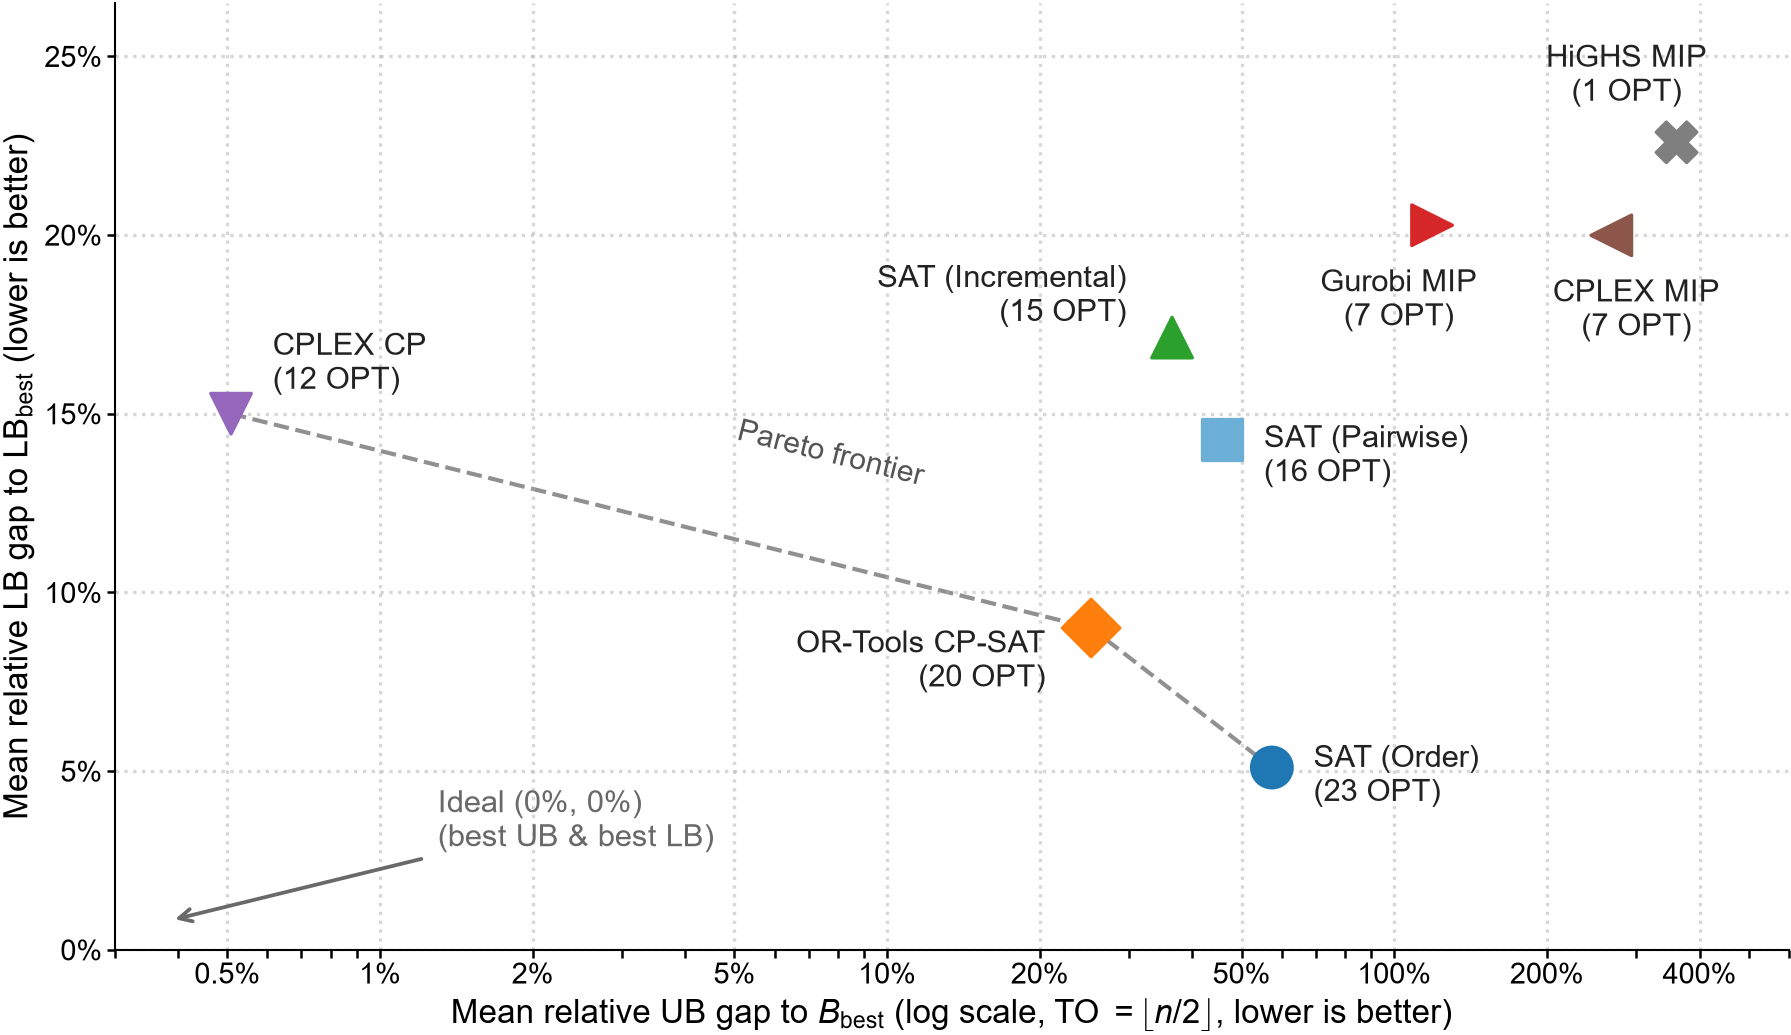
\includegraphics[width=0.92\linewidth]{figures/fig6_primal_dual.png}
    \caption{Primal--dual trade-off across all eight solvers over all 59 instances under rotation and reflection symmetry breaking. Horizontal axis: mean relative upper-bound excess over $B_{\text{best}}=\min_s B_s$ (log scale, imputing $\lfloor n/2\rfloor$ on TO, lower is better). Vertical axis: mean relative lower-bound shortfall below $\text{LB}_{\text{best}}=\max_s\text{LB}_s$ (lower is better). The dashed line marks the three-solver Pareto frontier.}
    \label{fig:primal_dual}
\end{figure}

Gurobi and CPLEX MIP certify the same 7 instances, all with at most 57 vertices. HiGHS certifies only \texttt{can\_24} and finds no labeling on 30 instances. The big-$M$ Constraints~(\ref{eq:mip_arc1}) and~(\ref{eq:mip_arc2}) yield a weak linear relaxation: setting $s_e=\tfrac12$ satisfies both constraints whenever $B\ge|d_e-n/2|$, and $d_e$ can also take fractional values through $w_e$, keeping the LP relaxation bound pinned at $L$. The empirical lower bounds confirm this mechanism directly: Gurobi and HiGHS never improve the dual bound above $L$ on any uncertified instance (0 non-OPT improvements, 20.3\% and 22.6\% LB gaps), CPLEX MIP does so only once (20.0\% LB gap), and their mean upper-bound excesses reach 118.8\% (Gurobi), 268.0\% (CPLEX MIP), and 360.3\% (HiGHS)---for example $B=48$ for Gurobi and $B=60$ for CPLEX MIP on \texttt{can\_144}, whose optimum is 7.

The order encoding finds no labeling on 9 instances, all with at least 132 vertices, including \texttt{bcsstk04}, \texttt{can\_187}, \texttt{dwt\_221}, \texttt{gre\_185}, \texttt{will199}, and the four \texttt{fs\_183} matrices. Separating CNF construction from solver time exposes the exact cause: on all 9 timeouts, CNF construction finishes in just 1.73--6.45~s (mean 3.9~s) and \texttt{solve\_calls} equals 1. Thus over 98\% of the 300~s budget is consumed inside the very first binary-search midpoint call, which often lands far from the optimum yet remains hard to satisfy in CaDiCaL (e.g., midpoint $B=48$ on \texttt{can\_187} where CPLEX CP finds $B=8$, or midpoint $B=57$ on \texttt{dwt\_221} where CPLEX CP finds $B=14$). The incremental scheme avoids this failure mode because its initial call has no distance clauses, returning a verified labeling on all 59 instances.

\subsection{Cactus Runtime Profile}

\begin{figure}[pos=htbp]
    \centering
    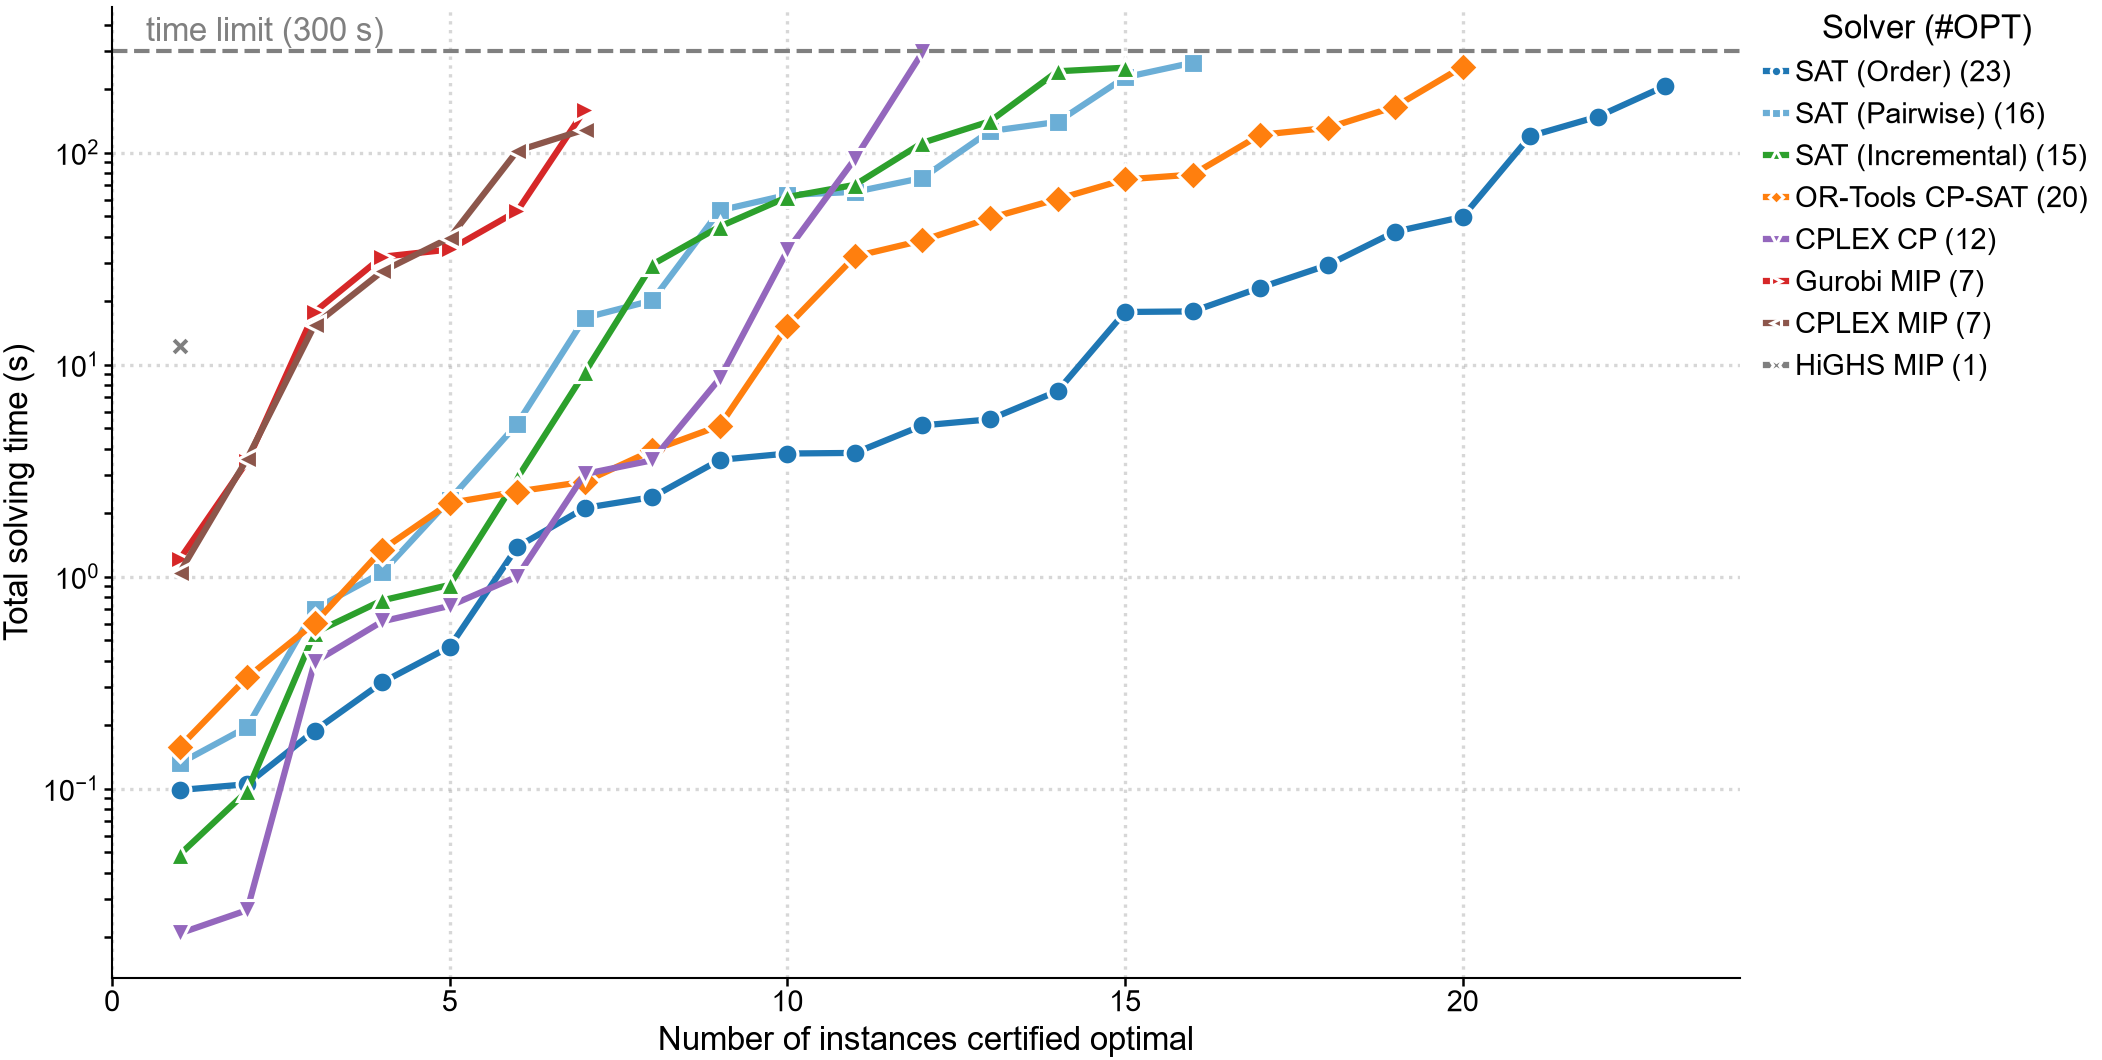
\includegraphics[width=0.95\linewidth]{figures/fig1_cactus_runtime.png}
    \caption{Cactus plot of the eight solvers with rotation and reflection symmetry breaking. A point $(k,t)$ means that the $k$-th fastest certified instance of a solver needed $t$ seconds. The number of certified instances is shown in parentheses.}
    \label{fig:cactus}
\end{figure}

Figure~\ref{fig:cactus} shows the cactus profile. The $x$-axis is the number of instances certified optimal, and the $y$-axis is the solving time on a logarithmic scale. Within 1~s, the order encoding, the incremental scheme, and CPLEX CP each certify 5 instances, while the pairwise encoding and CP-SAT certify 3. Within 30~s, the order encoding certifies 18 instances, compared with 10 for CP-SAT, 9 for CPLEX CP, and 8 for each pairwise scheme. The order encoding reaches 20 instances at 50~s and 23 at the 300~s limit, whereas CP-SAT reaches 20 and CPLEX CP 12. The MIP curves rise steeply after their first few instances.

\subsection{Binary Search Versus Incremental SAT and Encoding Overhead}

Table~\ref{tab:sat_schemes} and Figure~\ref{fig:sat_build_solve} dissect the three SAT approaches by separating Python/PySAT CNF construction time from CaDiCaL solving time and counting solver invocations. Unlike the CP and MIP baselines---whose model construction averages under 0.01~s for CP-SAT and CPLEX CP and at most 0.65~s for HiGHS---CNF generation represents a substantial share of certified runtime for the SAT pipelines: 21.3\% for SAT (Order), 18.4\% for SAT (Pairwise), and 10.8\% for SAT (Incremental).

\begin{table*}[pos=htbp]
\centering
\caption{CNF construction time, CaDiCaL solving time, and solver-call counts for the three SAT approaches under rotation and reflection symmetry breaking.}
\label{tab:sat_schemes}
\scriptsize
\setlength{\tabcolsep}{4pt}
\begin{tabular*}{\textwidth}{@{\extracolsep{\fill}}lccccccc@{}}
\toprule
\textbf{SAT Approach} & \makecell{\textbf{Mean Build}\\\textbf{All (s)}} & \makecell{\textbf{Max Build}\\\textbf{All (s)}} & \makecell{\textbf{Mean Build}\\\textbf{OPT (s)}} & \makecell{\textbf{Mean Solve}\\\textbf{OPT (s)}} & \makecell{\textbf{Build Share}\\\textbf{OPT (\%)}} & \makecell{\textbf{Mean Calls}\\\textbf{(OPT / All)}} & \textbf{OPT / TO} \\
\midrule
SAT (Order) & 5.82 & 52.46 & 3.03 & \textbf{26.97} & 21.3 & 4.5 / 3.2 & \textbf{23} / 9 \\
SAT (Pairwise) & 13.91 & 65.36 & 5.32 & 61.03 & 18.4 & \textbf{3.8} / \textbf{2.8} & 16 / 2 \\
SAT (Incremental) & \textbf{5.21} & \textbf{18.95} & \textbf{1.55} & 62.84 & \textbf{10.8} & 13.5 / 24.4 & 15 / \textbf{0} \\
\bottomrule
\end{tabular*}
\end{table*}

\begin{figure}[pos=htbp]
    \centering
    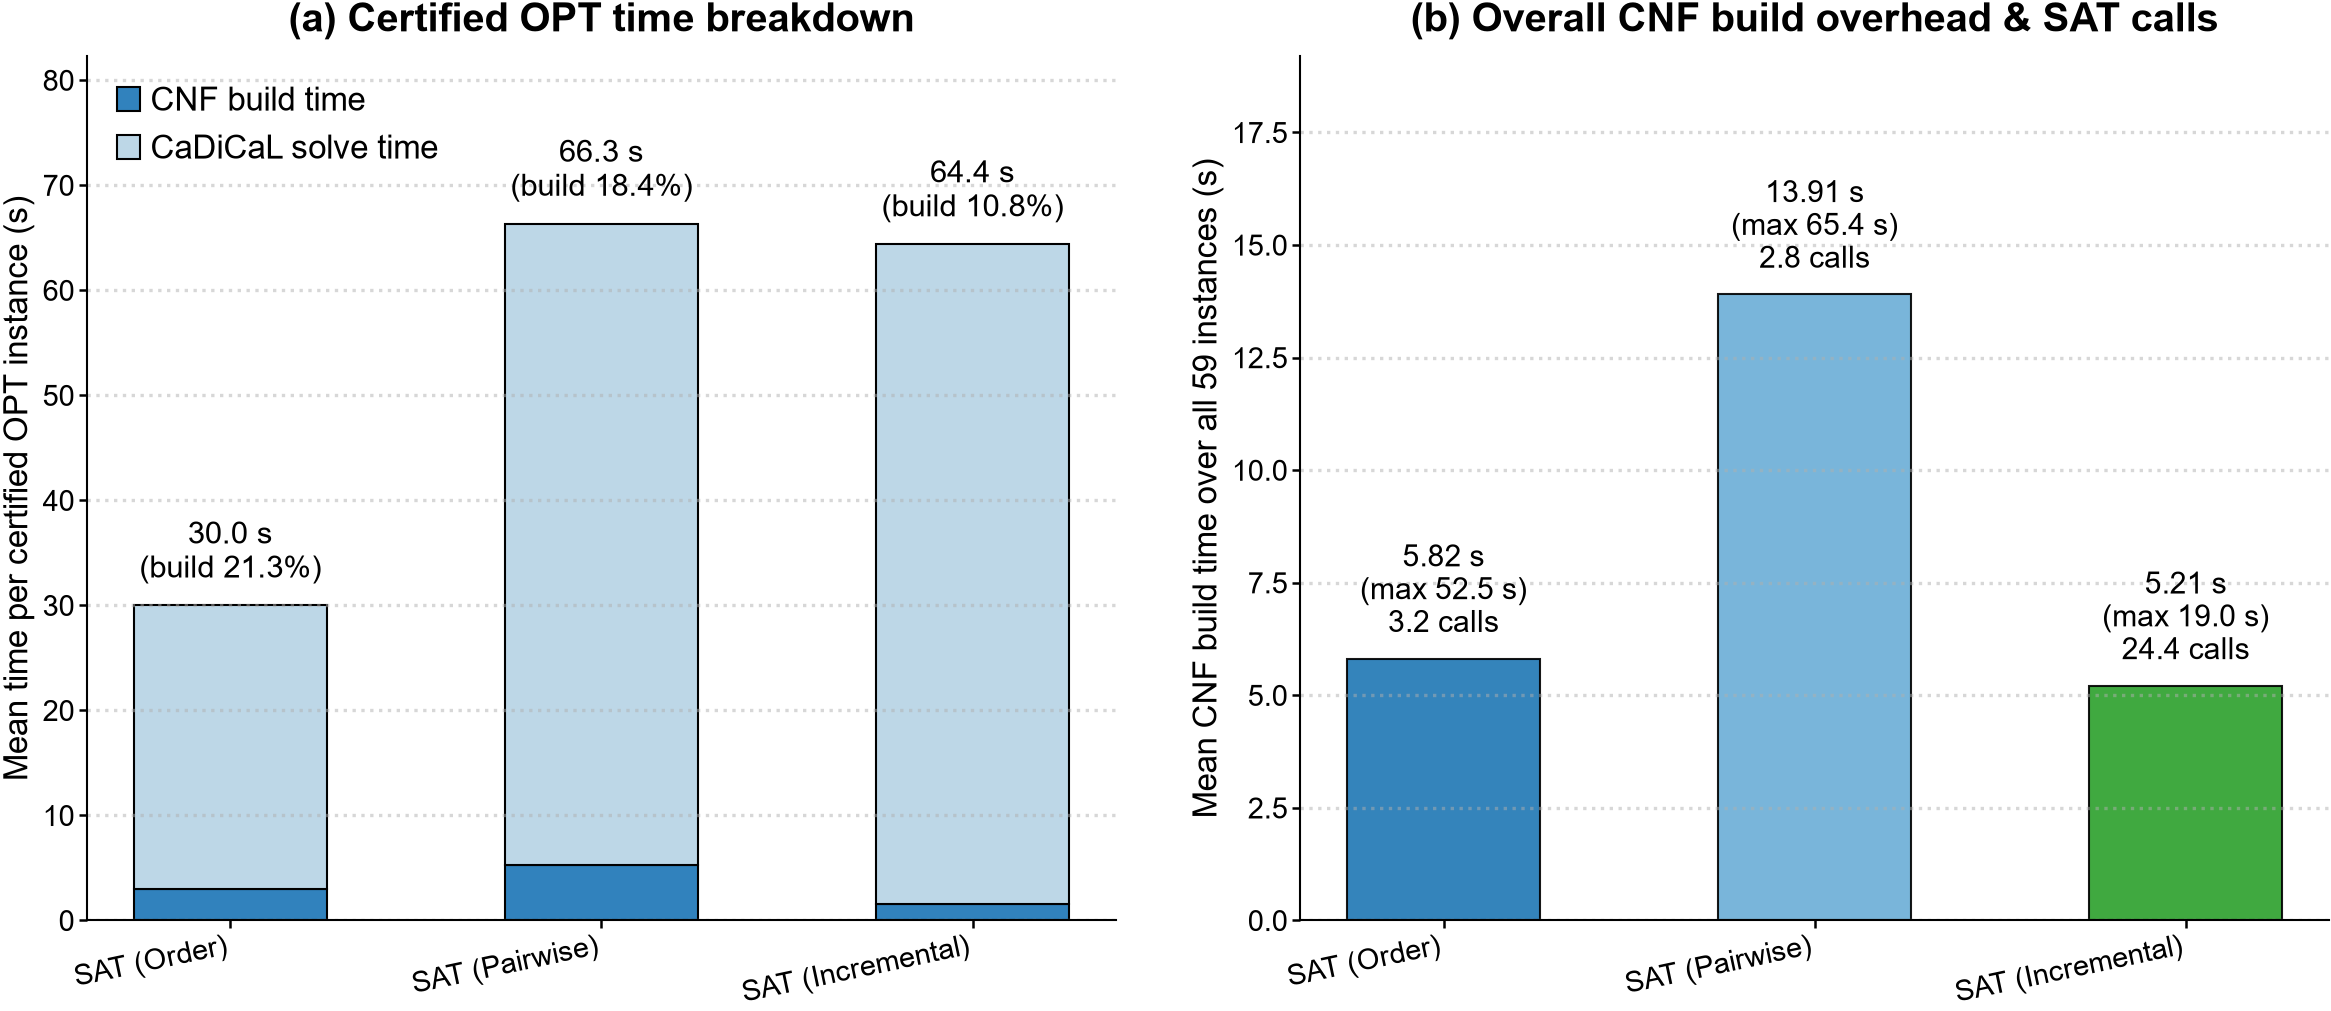
\includegraphics[width=0.95\linewidth]{figures/fig7_sat_build_solve.png}
    \caption{Encoding and search breakdown for the three SAT schemes: (a) mean CNF construction versus CaDiCaL solving time per certified optimal instance; (b) mean CNF build time and solver-call count across all 59 instances.}
    \label{fig:sat_build_solve}
\end{figure}

Comparing the two pairwise search schemes reveals a clean algorithmic trade-off. Because incremental descending search constructs the $\Theta(n^3)$ bijection formula $\mathcal{F}_{\text{bij}}$ only once and appends distance layers $\mathcal{D}_d$ monotonically, it reduces mean CNF build time across all 59 instances by 62.5\% (from 13.91~s to 5.21~s, and from 5.32~s to 1.55~s on certified instances). On the 15 instances certified by both pairwise schemes, incremental search is faster on 10, and across all 59 instances it obtains strictly smaller upper bounds than repeated binary search on 29 instances versus 9, with zero timeouts without a solution. The trade-off appears on instances whose optimum sits far below the initial feasible labeling: incremental search performs 13.5 solver calls on average for certified instances (24.4 overall, up to 28), whereas binary search needs only 3.8 calls. On \texttt{steam3} ($n=80$, $m=424$, $B^*=7$), repeated binary search jumps directly to $B^*=7$ in 5 calls and 16.61~s (7.04~s build + 9.57~s solve), while incremental descending search spends 28 calls and 300.02~s stalling at $B=13$. Furthermore, because incremental search never tests an unsatisfiable midpoint before reaching $B^*-1$, it yields zero lower-bound improvements on uncertified instances (Table~\ref{tab:overall_summary}).

\subsection{Impact of Symmetry Breaking}

\begin{figure}[pos=htbp]
    \centering
    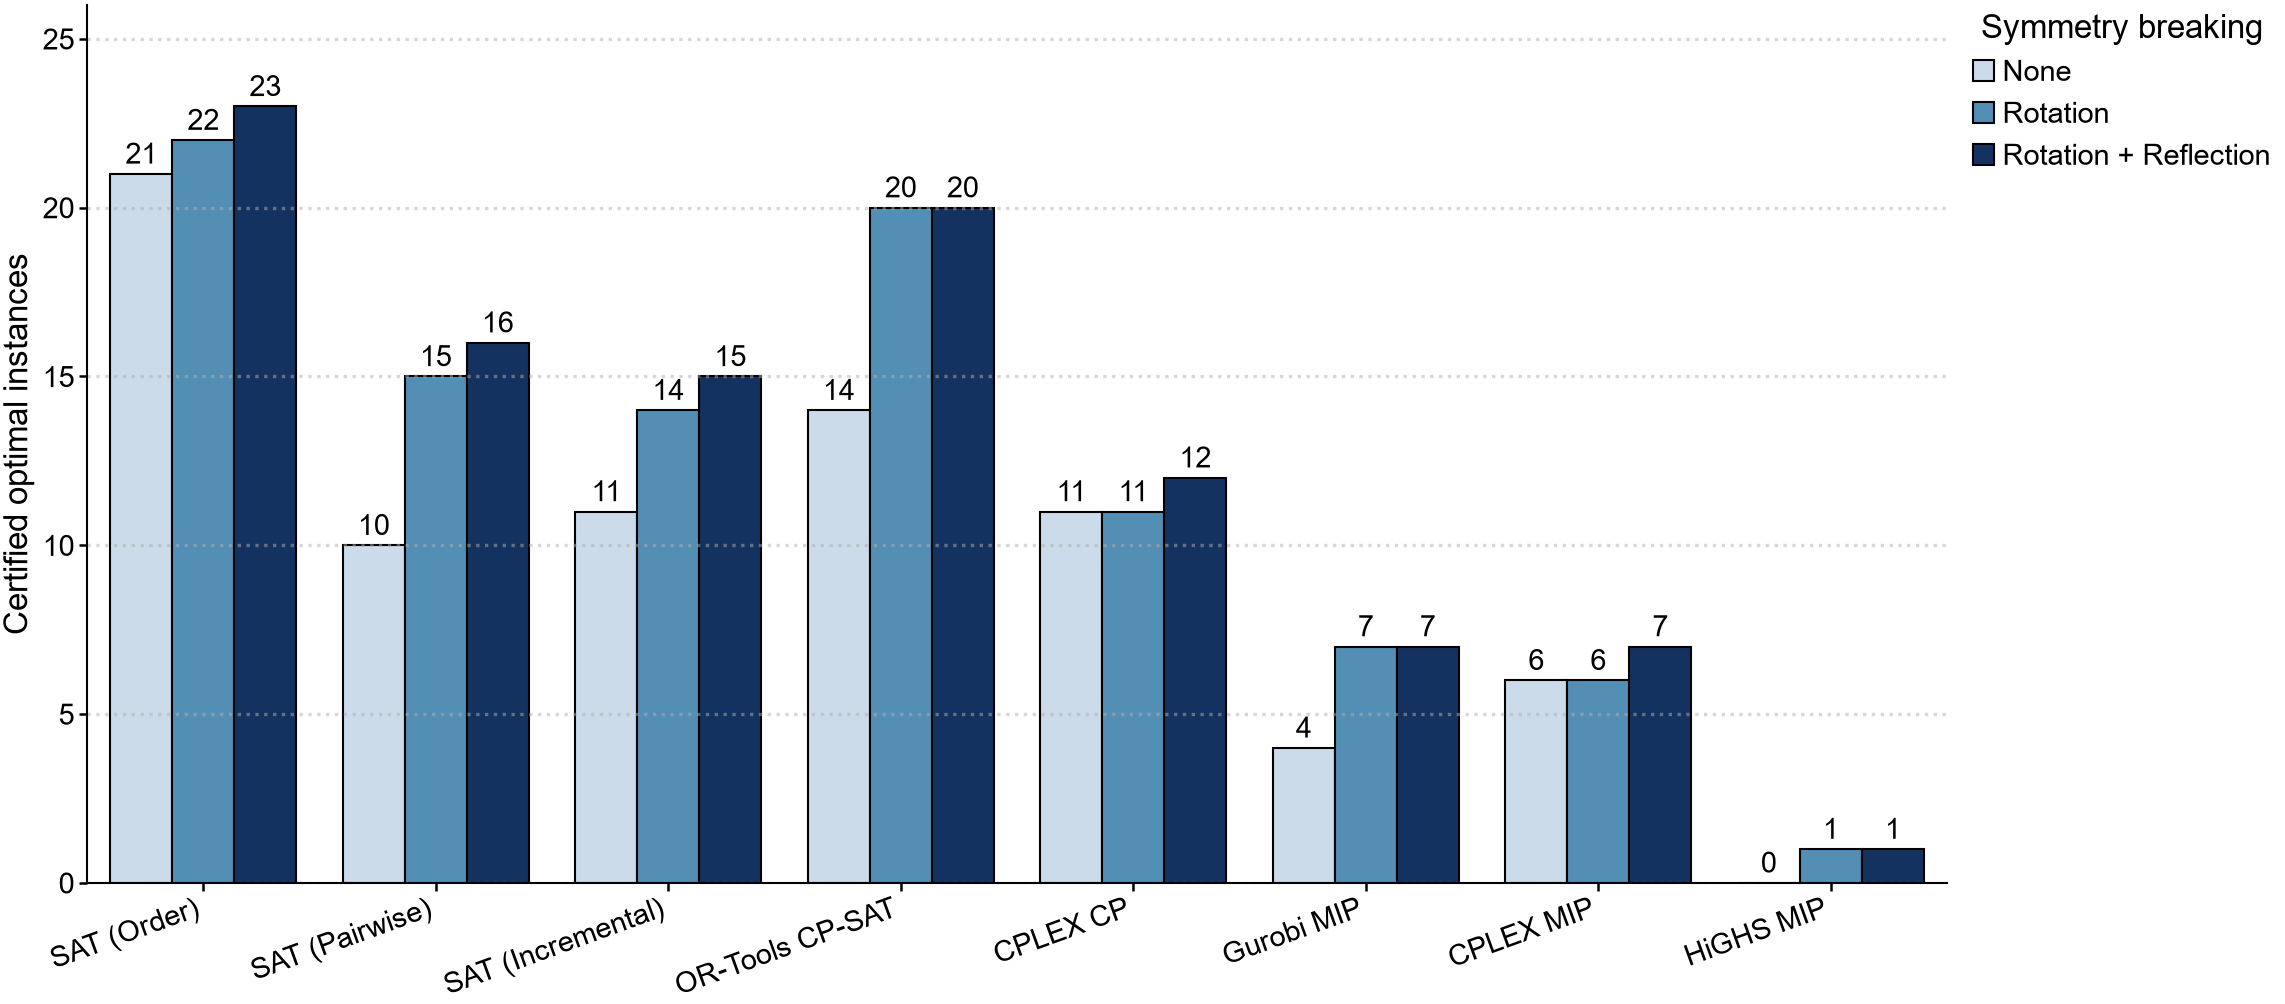
\includegraphics[width=0.95\linewidth]{figures/fig2_symmetry_impact.png}
    \caption{Number of certified optimal instances for all eight solvers under the three symmetry-breaking configurations: None, Rotation, and Rotation + Reflection.}
    \label{fig:symmetry}
\end{figure}

Figure~\ref{fig:symmetry} and Table~\ref{tab:symmetry_speedup} report both certification counts and runtime speedups across the three symmetry-breaking configurations. Rotation breaking accounts for most of the gain in certified instances, while reflection breaking adds at most one instance per solver. Beyond certifying additional graphs, symmetry breaking substantially accelerates instances already solved without it: geometric mean speedups on commonly certified instances (None to Rotation + Reflection) range from 1.84$\times$ for SAT (Order) to 4.38$\times$ for SAT (Incremental) and 7.02$\times$ for Gurobi MIP.

\begin{table*}[pos=htbp]
\centering
\caption{Impact of symmetry breaking across all eight solvers: certified optimal counts under None, Rotation (Rot.), and Rotation + Reflection (Rot.+Refl.), number of instances certified under both None and Rot.+Refl.\ (\#Common), and geometric mean and maximum runtime speedups ($t_{\text{None}}/t_{\text{Rot.+Refl.}}$) on those common instances.}
\label{tab:symmetry_speedup}
\scriptsize
\begin{tabular*}{\textwidth}{@{\extracolsep{\fill}}lcccccl@{}}
\toprule
\textbf{Solver} & \textbf{None} & \textbf{Rot.} & \textbf{Rot.+Refl.} & \textbf{\#Common} & \textbf{Geom.\ Speedup} & \textbf{Max Speedup (Instance)} \\
\midrule
SAT (Order) & 21 & 22 & 23 & 21 & 1.84$\times$ & 5.95$\times$ (\texttt{nos4}: 251.99~s $\to$ 42.35~s) \\
OR-Tools CP-SAT & 14 & 20 & 20 & 14 & 2.00$\times$ & 21.00$\times$ (\texttt{ibm32}: 52.86~s $\to$ 2.52~s) \\
SAT (Pairwise) & 10 & 15 & 16 & 10 & 2.45$\times$ & 52.52$\times$ (\texttt{pores\_1}: 36.92~s $\to$ 0.70~s) \\
SAT (Incremental) & 11 & 14 & 15 & 11 & 4.38$\times$ & 94.04$\times$ (\texttt{ibm32}: 72.61~s $\to$ 0.77~s) \\
CPLEX CP & 11 & 11 & 12 & 11 & 3.36$\times$ & 26.16$\times$ (\texttt{steam3}: 225.34~s $\to$ 8.61~s) \\
Gurobi MIP & 4 & 7 & 7 & 3 & 7.02$\times$ & 38.48$\times$ (\texttt{lap\_25}: 134.44~s $\to$ 3.49~s) \\
CPLEX MIP & 6 & 6 & 7 & 6 & 1.09$\times$ & 2.16$\times$ (\texttt{can\_24}: 2.26~s $\to$ 1.04~s) \\
HiGHS MIP & 0 & 1 & 1 & 0 & -- & -- (certifies \texttt{can\_24} in 12.18~s) \\
\bottomrule
\end{tabular*}
\end{table*}

\begin{itemize}
    \item SAT (Pairwise) increases from 10 (None) to 15 (Rotation) and 16 (Rotation + Reflection), a 60\% gain, with a 2.45$\times$ geometric mean speedup (up to 52.52$\times$ on \texttt{pores\_1}).
    \item SAT (Incremental) increases from 11 to 14 and 15 (+36\%) and achieves the largest SAT speedup (4.38$\times$ geometric mean, 94.04$\times$ on \texttt{ibm32}).
    \item OR-Tools CP-SAT increases from 14 to 20 under both restricted configurations (+43\%) with a 2.00$\times$ geometric mean speedup.
    \item SAT (Order) increases from 21 to 22 and 23 (+10\%) with a 1.84$\times$ geometric mean speedup; its certification count gain is smaller because the order encoding already certifies most of these instances without symmetry breaking.
    \item CPLEX CP gains one certification with reflection breaking (11 to 12) yet accelerates by 3.36$\times$ on common instances (26.16$\times$ on \texttt{steam3}). CPLEX MIP rises from 6 to 7 (1.09$\times$), HiGHS rises from 0 to 1, and Gurobi rises from 4 to 7 with a 7.02$\times$ geometric mean speedup on the 3 instances solved in both modes. Notably, Gurobi is the only solver that exhibits a single regression under symmetry breaking: it certifies \texttt{dwt\_66} ($B^*=3$) in 104.34~s under None, but stalls at $B=5$ (300.00~s) when explicit symmetry constraints are added, reflecting a known interaction in MIP solvers where static symmetry constraints can disrupt built-in presolve and orbital branching.
\end{itemize}
Fixing $\phi(a)=1$ removes the $n$ rotations of each labeling, and the reflection restriction halves the remaining space. The gain is largest for the encodings that rely on unsatisfiability proofs, because without these restrictions the solver must refute up to $2n$ symmetric copies of each partial labeling.

\subsection{Bandwidth Quality on Representative Instances}

\begin{figure}[pos=htbp]
    \centering
    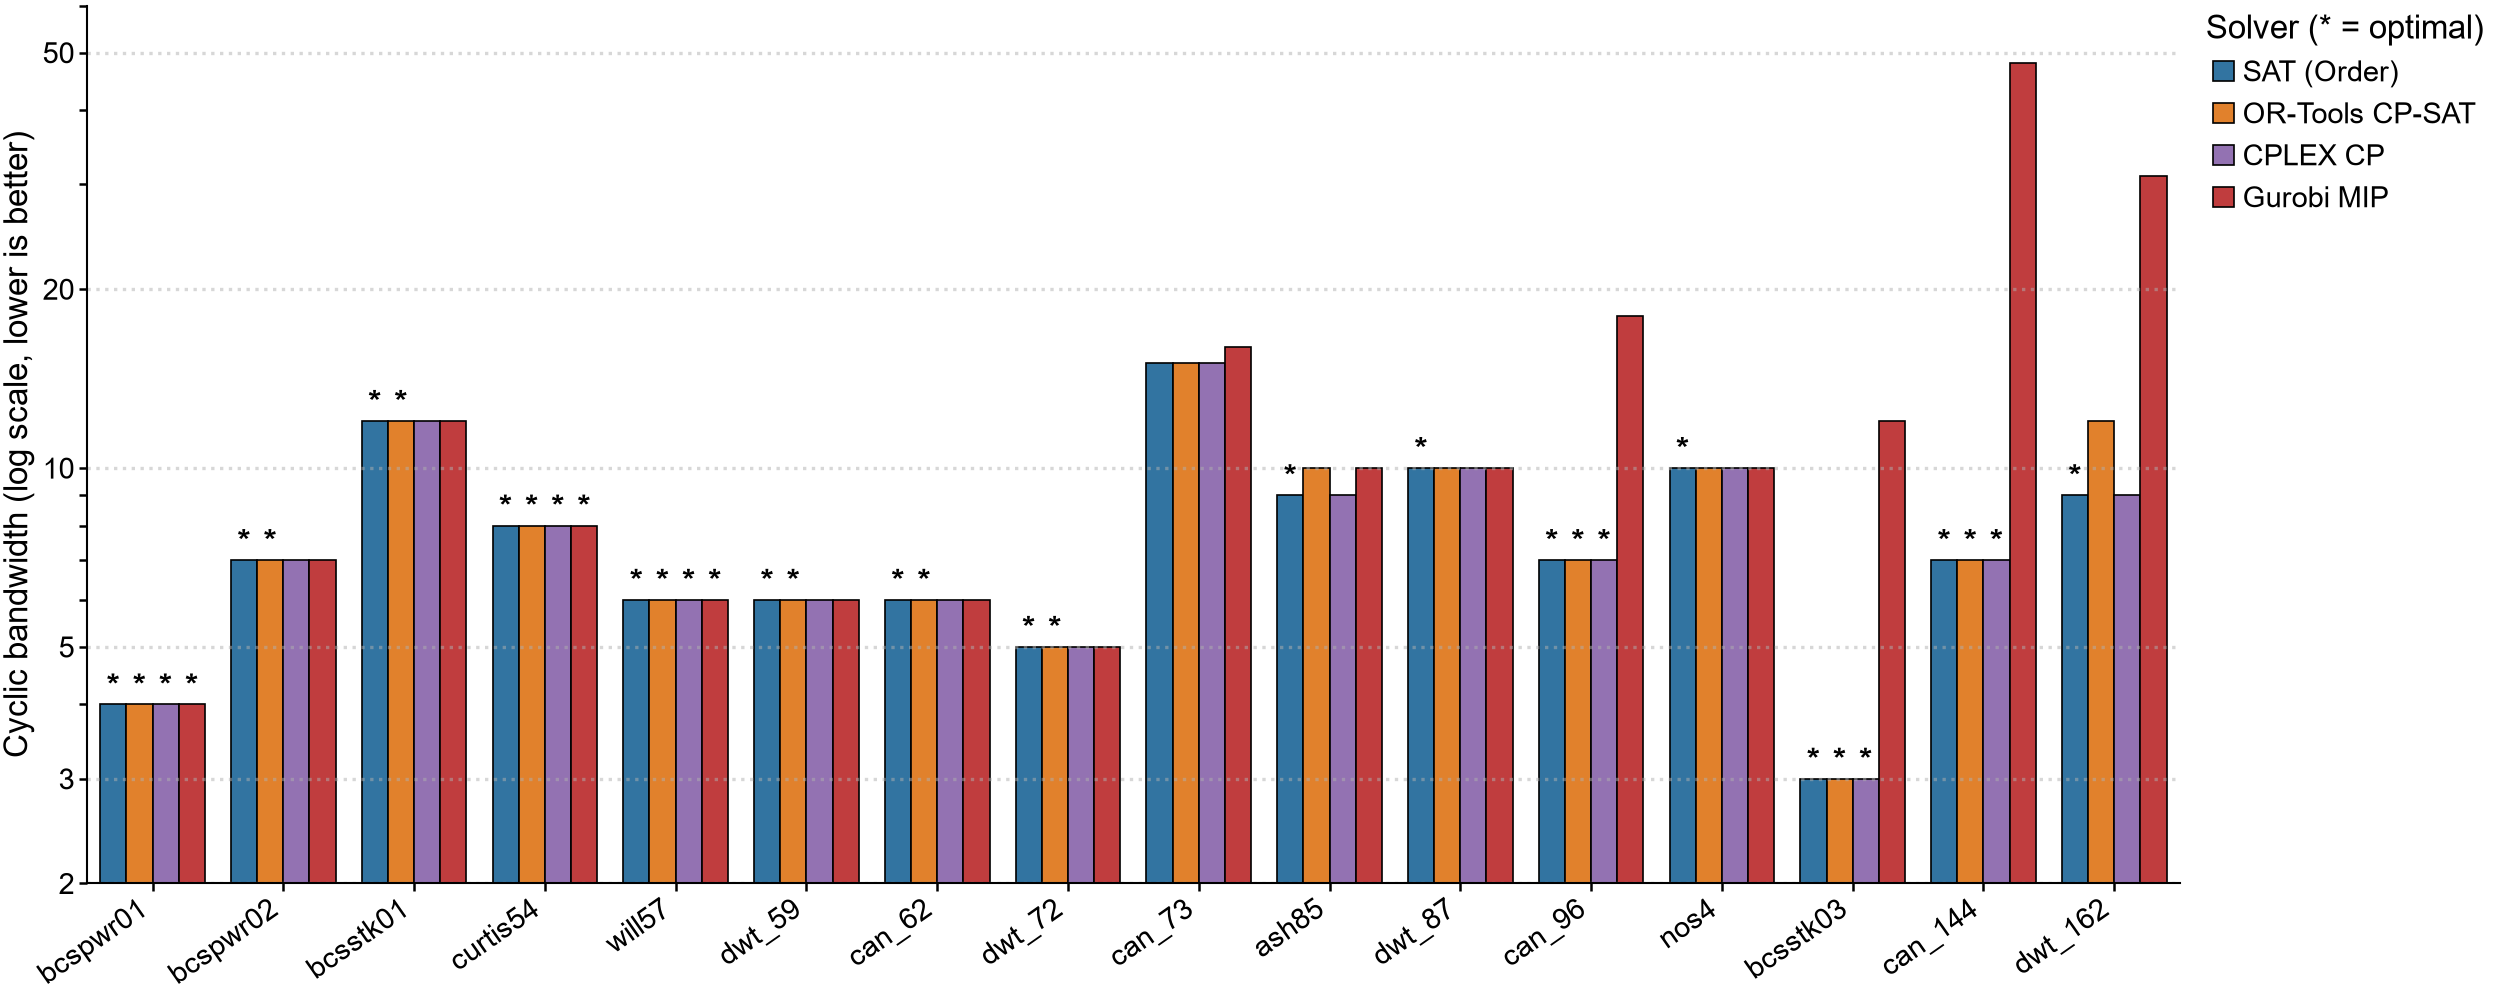
\includegraphics[width=0.98\linewidth]{figures/fig3_bandwidth_comparison.png}
    \caption{Cyclic bandwidth returned by SAT (Order), OR-Tools CP-SAT, CPLEX CP, and Gurobi MIP on 16 representative Harwell--Boeing instances (logarithmic scale). A star (*) marks a certified optimal value.}
    \label{fig:bandwidth}
\end{figure}

Figure~\ref{fig:bandwidth} compares the bandwidths returned by four solvers on 16 instances. On the eight smallest instances in the figure, from \texttt{bcspwr01} to \texttt{dwt\_72} ($n\le72$), the four solvers return the same bandwidth, although not all of them certify it. For example, all four return $B=7$ on \texttt{bcspwr02}, but only the order encoding (3.83~s) and CP-SAT (254.21~s) certify it. On larger instances the results differ.
\begin{itemize}
    \item On \texttt{ash85} ($n=85$, $m=219$), the order encoding certifies $B^*=9$ in 17.71~s. CPLEX CP also finds $B=9$ without a proof, while CP-SAT and Gurobi return $B=10$.
    \item On \texttt{bcsstk03} ($n=112$, $m=264$), the order encoding, CP-SAT, and CPLEX CP certify $B^*=3$ in 5.52~s, 32.38~s, and 1.00~s, respectively, while Gurobi returns $B=12$.
    \item On \texttt{can\_144} ($n=144$, $m=576$), the order encoding, CP-SAT, and CPLEX CP certify $B^*=7$, while Gurobi returns $B=48$.
    \item On \texttt{dwt\_162} ($n=162$, $m=510$), the order encoding certifies $B^*=9$ in 119.60~s, CPLEX CP finds $B=9$ without a proof, CP-SAT returns 12, and Gurobi returns 31.
\end{itemize}

\subsection{Pairwise Comparison: SAT (Order) and OR-Tools CP-SAT}

\begin{figure}[pos=htbp]
    \centering
    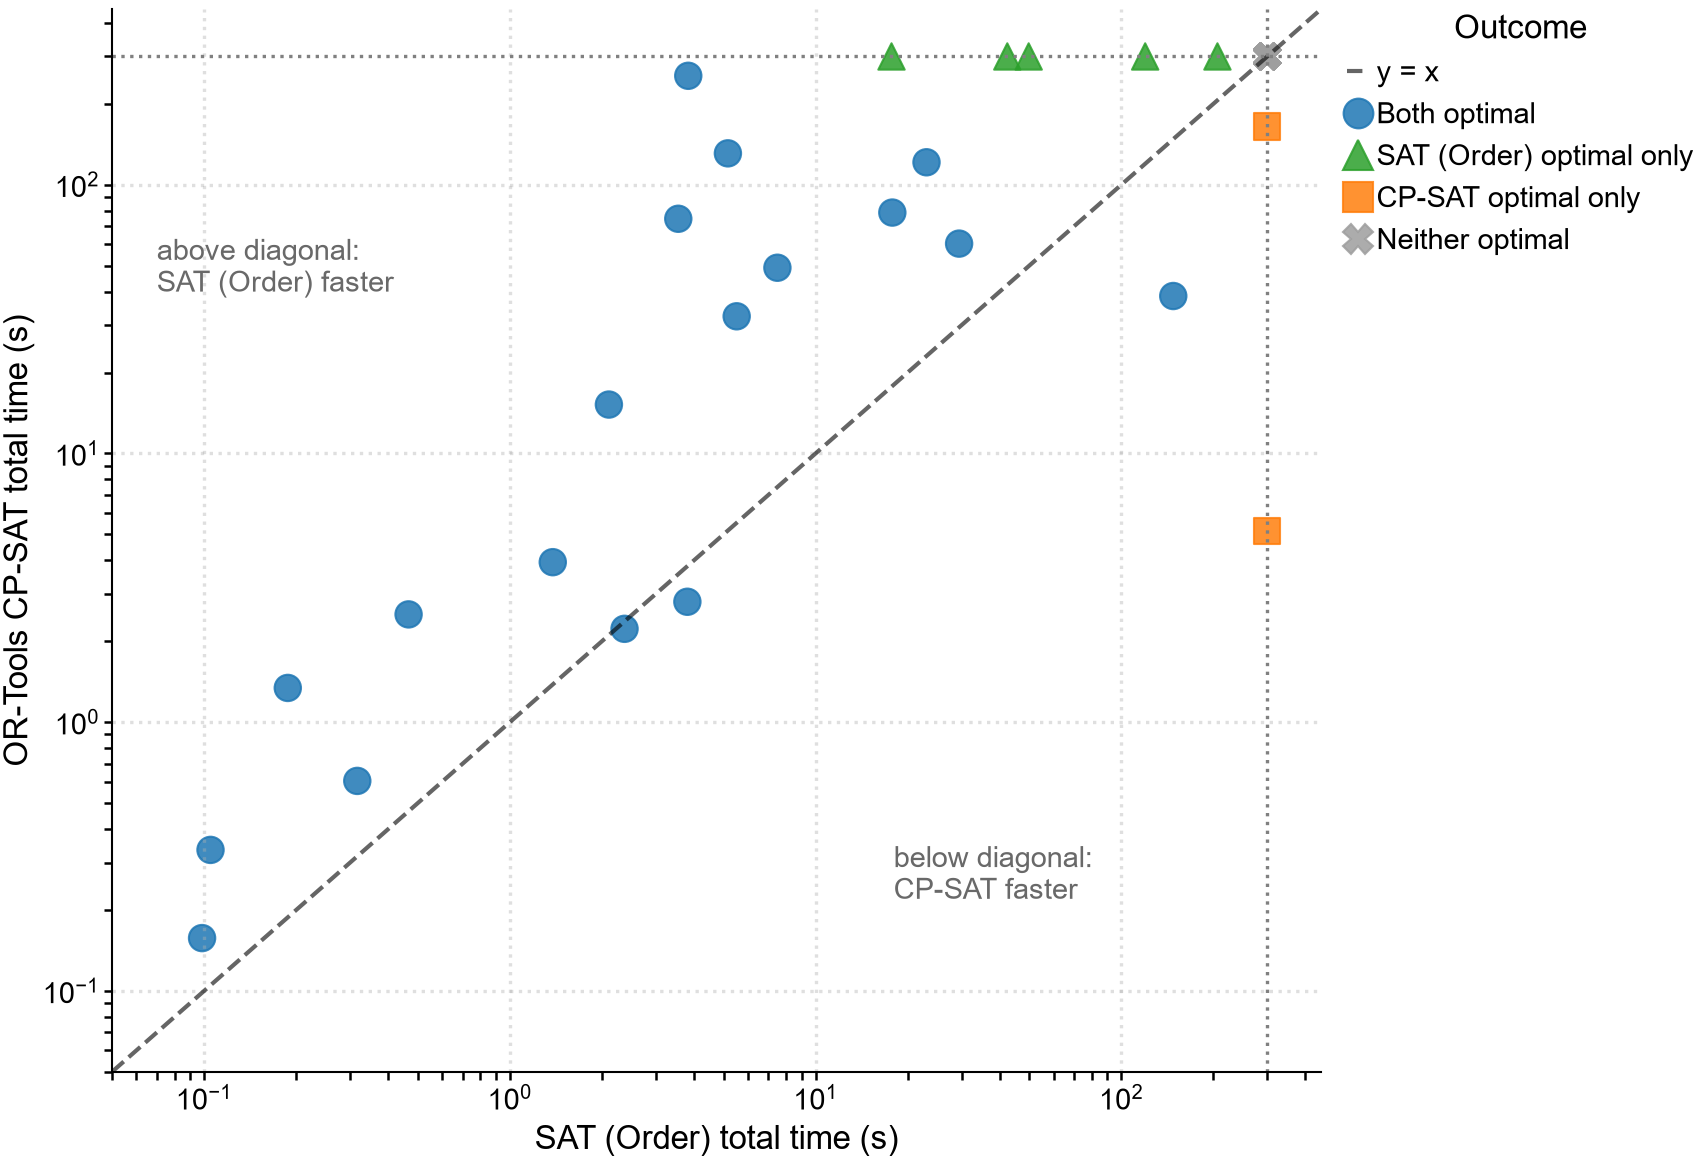
\includegraphics[width=0.75\linewidth]{figures/fig4_scatter_sat_vs_cpsat.png}
    \caption{Total solving time of SAT (Order) ($x$-axis) and OR-Tools CP-SAT ($y$-axis) on all 59 instances (log--log scale). Points above the dashed diagonal $y=x$ are instances on which SAT (Order) is faster. Runs that reach the limit are drawn at 300~s.}
    \label{fig:scatter}
\end{figure}

Figure~\ref{fig:scatter} compares the order encoding with CP-SAT, the strongest baseline in terms of certified instances. Both solvers certify 18 common instances. On 15 of them the order encoding is faster, for example \texttt{bcspwr01} (0.32~s versus 0.60~s), \texttt{bcsstk01} (7.50~s versus 49.08~s), and \texttt{can\_61} (29.46~s versus 60.35~s). CP-SAT is faster on \texttt{curtis54}, \texttt{dwt\_66}, and \texttt{can\_144}. The order encoding alone certifies five instances (\texttt{ash85}, \texttt{dwt\_87}, \texttt{nos4}, \texttt{dwt\_162}, and \texttt{dwt\_198}), and CP-SAT alone certifies two (\texttt{arc130} and \texttt{nos1}). CP-SAT often returns the better upper bound on uncertified instances: over all 59 instances, it returns a smaller bandwidth than the order encoding on 26, including the 9 on which the order encoding finds no labeling.

\subsection{Scaling with Instance Size and Graph Structure}

\begin{figure}[pos=htbp]
    \centering
    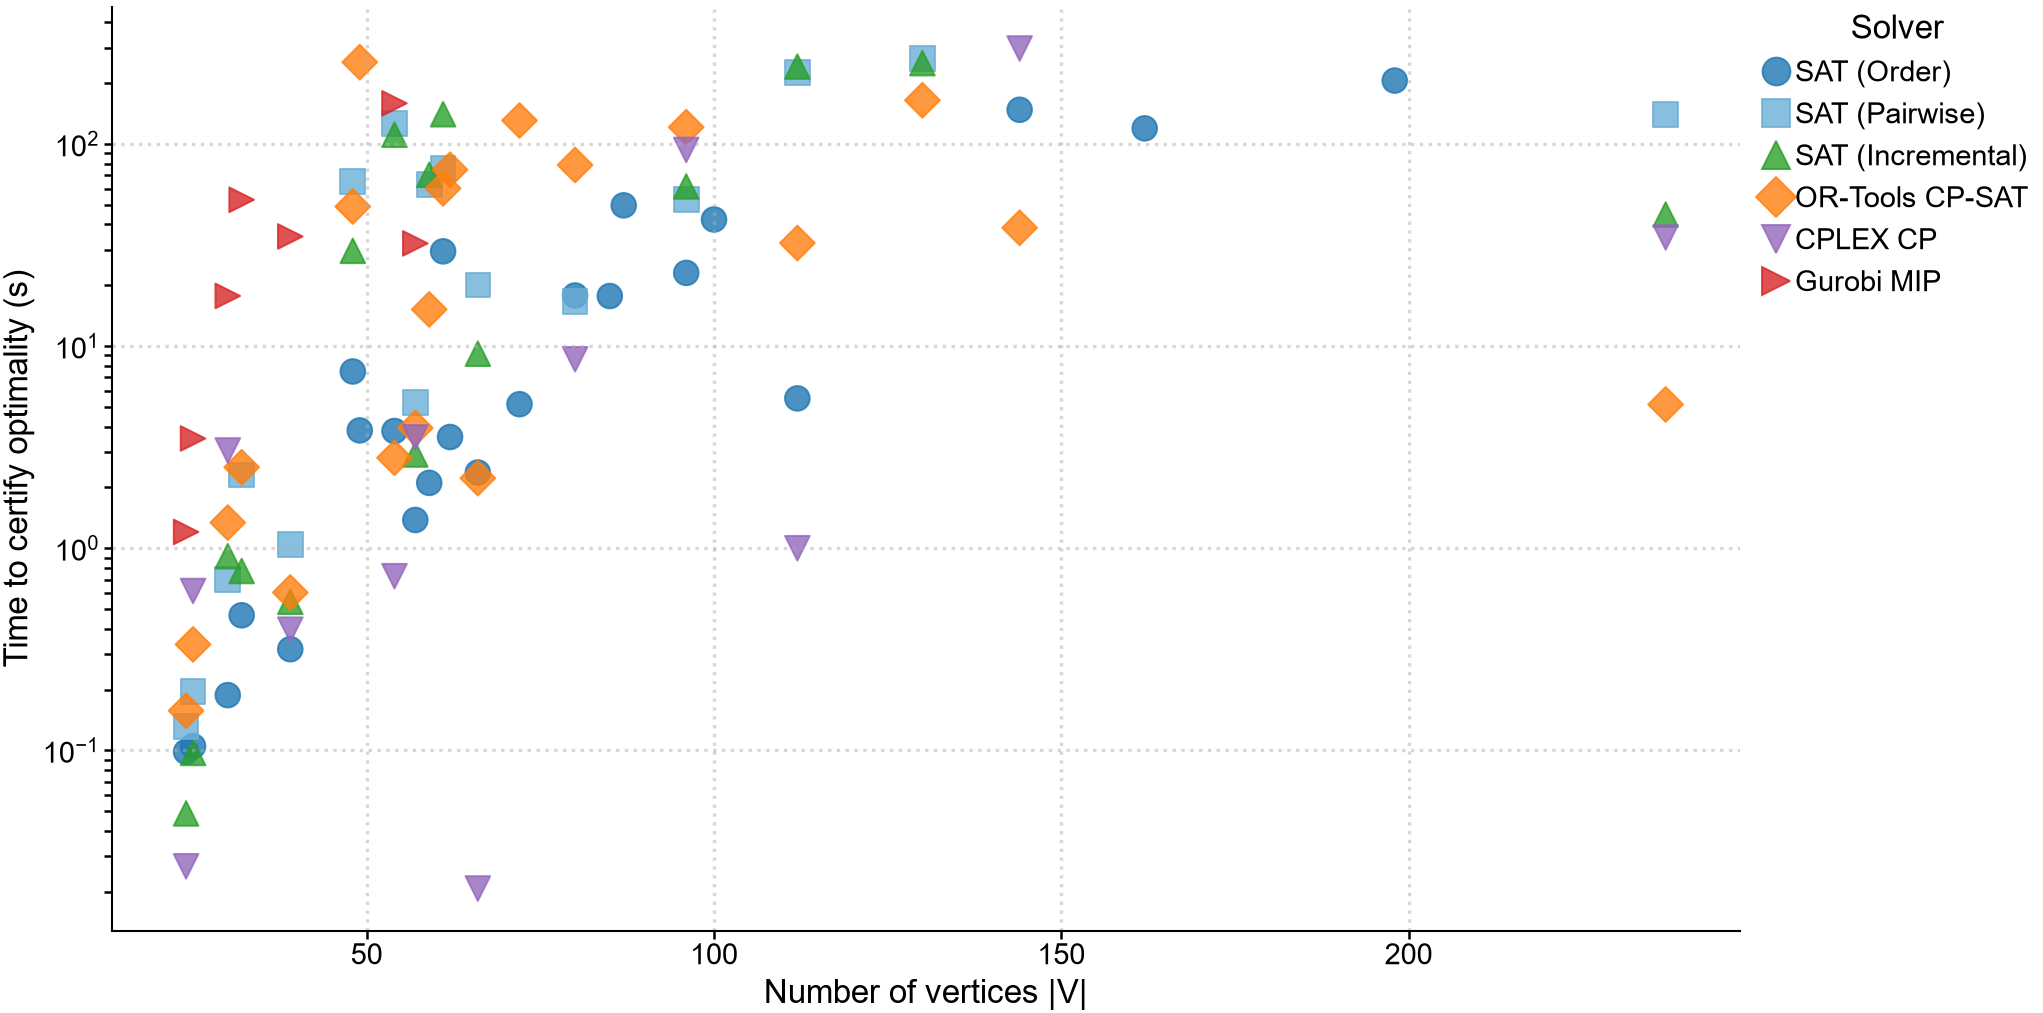
\includegraphics[width=0.95\linewidth]{figures/fig5_scaling.png}
    \caption{Time to certify optimality as a function of the number of vertices $|V|$ for the instances certified by six solvers.}
    \label{fig:scaling}
\end{figure}

Figure~\ref{fig:scaling} plots the time to certify optimality against the number of vertices. Gurobi and CPLEX MIP certify no instance with more than 57 vertices. The order encoding certifies instances up to $n=198$ (\texttt{dwt\_198}, $B^*=8$). The pairwise schemes, CP-SAT, and CPLEX CP certify \texttt{nos1} with $n=237$, which has a small optimum $B^*=3$.

Instance size alone therefore does not determine difficulty; the tightness of the optimum relative to the degree lower bound $L=\lceil\Delta(G)/2\rceil$ is a much stronger separator. Across the 25 VBS-certified instances, the median graph has $n=66$, $m=176$, optimal bandwidth $B^*=7$, and a tightness ratio $B^*/L=1.50$ (with four instances achieving $B^*=L$ exactly: \texttt{curtis54}, \texttt{dwt\_66}, \texttt{bcsstk03}, and \texttt{can\_144}). By contrast, across the 34 uncertified instances, the median graph has $n=164$, $m=608$, best-found upper bound $B=23$, and ratio $B/L=2.75$. When $B^*$ sits close to $L$, high-degree neighborhoods leave almost no slack on the cycle, enabling strong unit propagation and \textsc{AllDifferent} filtering even at $n=237$; when $B/L$ is large---as in \texttt{bcsstk04} ($n=132$, $m=1758$, $L=23$, best $B=38$)---local degree constraints stay loose and global graph topology dominates search.

\section{Conclusion}
\label{sec:conclusion}

This paper studied exact methods for the Cyclic Bandwidth Minimization Problem. We formulated a pairwise and an order SAT encoding of the CBMP decision problem, solved them by repeated SAT calls with binary search and, for the pairwise encoding, by an incremental descending search, and removed the rotation and reflection symmetries of the host cycle. We compared these methods with CPLEX CP, OR-Tools CP-SAT, Gurobi, CPLEX MIP, and HiGHS on 59 Harwell--Boeing instances under a 300~s limit.

The main findings are the following.
\begin{enumerate}
    \item The order encoding certifies the largest number of instances (23, median 5.16~s) and delivers the strongest average lower-bound tightening ($+1.71$ above $L$), followed by CP-SAT (20), the pairwise encoding (16), incremental pairwise SAT (15), and CPLEX CP (12). Together, SAT (Order) and CP-SAT recover the full 25-instance virtual best solver, whereas MIP solvers certify at most 7 instances (all with $n\le57$) and rarely tighten the LP relaxation above $L$.
    \item Certification and upper bounds exhibit a stark primal--dual split. CPLEX CP returns the best upper bound on 57 of 59 instances with a mean relative excess of only 0.5\%, while SAT (Order) times out on its single first binary-search midpoint call on 9 large instances despite finishing CNF construction in under 6.5~s.
    \item Incremental descending search reduces pairwise CNF construction overhead by 62.5\%, accelerates 10 of 15 commonly certified instances, and yields tighter upper bounds than binary pairwise search on 29 instances with zero timeouts, though linear descent can stall when $B^*$ is far below the initial labeling (e.g., \texttt{steam3}).
    \item Symmetry breaking---primarily rotation breaking---increases certified instances by up to 60\% for pairwise SAT and 43\% for CP-SAT, while delivering 1.84$\times$ to 4.38$\times$ geometric mean speedups across SAT and CP solvers (and up to 94.04$\times$ on individual graphs).
    \item Tractability tracks the ratio $B^*/L$ alongside graph size: certified graphs have median $B^*/L=1.50$, whereas uncertified graphs have median $B/L=2.75$.
\end{enumerate}

The study has limitations. The largest instance has 245 vertices, because the pairwise encoding grows as $\Theta(m\,n^2)$ and larger matrices were excluded. In addition, the SAT solvers ran on a single thread whereas the CP and MIP baselines used 8 threads; this asymmetry makes the optimality lead of the order encoding noteworthy, though a uniform single-threaded comparison and parallel SAT portfolios remain to be evaluated. Only the pairwise AMO encoding and the sequential counter were evaluated, although the implementation also supports the other PySAT cardinality encodings. Future work will evaluate these encodings, pair CPLEX CP's fast upper bounds (or heuristics such as NILS~\citep{ren2020nils}) as a warm start to eliminate the first-midpoint timeout bottleneck of SAT (Order), and develop an incremental variant of the order encoding.

\section*{CRediT Authorship Contribution Statement}
\textbf{Truong Dinh Duc}: Conceptualization, Methodology, Software (SAT encodings, search algorithms, and baseline formulations), Validation.
\textbf{Hoang Minh Duc}: Methodology, Software (benchmark runner), Investigation, Data Curation.
\textbf{Le Trung Hieu}: Software (visualization and plotting scripts), Formal Analysis, Writing -- Original Draft, Writing -- Review \& Editing.

\section*{Declaration of Competing Interest}
The authors declare that they have no known competing financial interests or personal relationships that could have appeared to influence the work reported in this paper.

\section*{Data Availability}
The source code, benchmark instances, result CSV files, and visualization scripts used in this paper are openly available in the GitHub repository \url{https://github.com/missos1/CBMP-SAT-CP-MIP_ILP}.

\appendix
\section{Detailed Benchmark Results}
\label{app:results}

Tables~\ref{tab:detailed_results_part1} and~\ref{tab:detailed_results_part2} report the results of six solvers on all 59 instances with rotation and reflection symmetry breaking. The results of CPLEX MIP and HiGHS, and of the other symmetry-breaking configurations, are available in the repository listed in the Data Availability section.

\begin{table*}[pos=htbp]
\centering
\caption{Detailed results on the 59 Harwell--Boeing instances with rotation and reflection symmetry breaking and a 300~s limit, Part~1 (instances 1--30 in alphabetical order). A value with an asterisk (*) is a certified optimum, followed by the total time in seconds; (FEAS) marks a verified labeling without optimality proof; -- (TO) means that no labeling was found.}
\label{tab:detailed_results_part1}
\scriptsize
\begin{tabular*}{\textwidth}{@{\extracolsep{\fill}}lrrllllll@{}}
\toprule
\textbf{Instance} & \textbf{$|V|$} & \textbf{$|E|$} & \textbf{SAT (Order)} & \textbf{SAT (Pairwise)} & \textbf{SAT (Incr.)} & \textbf{OR-Tools CP-SAT} & \textbf{CPLEX CP} & \textbf{Gurobi MIP} \\
\midrule
\tableinput{table_instances_part1.tex}
\bottomrule
\end{tabular*}
\end{table*}

\begin{table*}[pos=htbp]
\centering
\caption{Detailed results on the 59 Harwell--Boeing instances, Part~2 (instances 31--59). Notation as in Table~\ref{tab:detailed_results_part1}.}
\label{tab:detailed_results_part2}
\scriptsize
\begin{tabular*}{\textwidth}{@{\extracolsep{\fill}}lrrllllll@{}}
\toprule
\textbf{Instance} & \textbf{$|V|$} & \textbf{$|E|$} & \textbf{SAT (Order)} & \textbf{SAT (Pairwise)} & \textbf{SAT (Incr.)} & \textbf{OR-Tools CP-SAT} & \textbf{CPLEX CP} & \textbf{Gurobi MIP} \\
\midrule
\tableinput{table_instances_part2.tex}
\bottomrule
\end{tabular*}
\end{table*}

\bibliographystyle{model1-num-names}
\newpage
\bibliography{cas-refs}

\end{document}
